%%%%%%%%%%%%%%%%%%%%%%%%%%%%%%%%%%%%%%%%%%%%%%%%%%%%%%%%%%%%%%%
%% OXFORD THESIS TEMPLATE

% Use this template to produce a standard thesis that meets the Oxford University requirements for DPhil submission
%
% Originally by Keith A. Gillow (gillow@maths.ox.ac.uk), 1997
% Modified by Sam Evans (sam@samuelevansresearch.org), 2007
% Modified by John McManigle (john@oxfordechoes.com), 2015
% Modified by Ulrik Lyngs (ulrik.lyngs@cs.ox.ac.uk), 2018-, for use with R Markdown
%
% Ulrik Lyngs, 25 Nov 2018: Following John McManigle, broad permissions are granted to use, modify, and distribute this software
% as specified in the MIT License included in this distribution's LICENSE file.
%
% John commented this file extensively, so read through to see how to use the various options.  Remember that in LaTeX,
% any line starting with a % is NOT executed.  Several places below, you have a choice of which line to use
% out of multiple options (eg draft vs final, for PDF vs for binding, etc.)  When you pick one, add a % to the beginning of
% the lines you don't want.


%%%%% PAGE LAYOUT
% The most common choices should be below.  You can also do other things, like replacing "a4paper" with "letterpaper", etc.

% This one formats for two-sided binding (ie left and right pages have mirror margins; blank pages inserted where needed):
%\documentclass[a4paper,twoside]{templates/ociamthesis}
% This one formats for one-sided binding (ie left margin > right margin; no extra blank pages):
%\documentclass[a4paper]{ociamthesis}
% This one formats for PDF output (ie equal margins, no extra blank pages):
%\documentclass[a4paper,nobind]{templates/ociamthesis}

% As you can see from the uncommented line below, oxforddown template uses the a4paper size, 
% and passes in the binding option from the YAML header in index.Rmd:
\documentclass[a4paper, twoside]{templates/ociamthesis}


%%%%% ADDING LATEX PACKAGES
% add hyperref package with options from YAML %

%%%%%%%%%%%%%
% TIPOGRAFÍA 
%%%%%%%%%%%%%
\usepackage{libertinus} % Fuente LIBERTINE Linux
%%
\usepackage[pdfpagelabels]{hyperref}
% change the default coloring of links to something sensible
\usepackage{xcolor}
\definecolor{myurlcolor}{RGB}{0,0,139}
\definecolor{mycitecolor}{RGB}{0,33,71}

\hypersetup{
  hidelinks,
  colorlinks,
  linkcolor=.,
  urlcolor=myurlcolor,
  citecolor=mycitecolor
}



% add float package to allow manual control of figure positioning %
\usepackage{float}

% enable strikethrough
\usepackage[normalem]{ulem}

% use soul package for correction highlighting
\usepackage{color, soul}
\definecolor{correctioncolor}{HTML}{CCCCFF}
\sethlcolor{correctioncolor}
\newcommand{\ctext}[3][RGB]{%
  \begingroup
  \definecolor{hlcolor}{#1}{#2}\sethlcolor{hlcolor}%
  \hl{#3}%
  \endgroup
}
\soulregister\ref7
\soulregister\cite7
\soulregister\autocite7
\soulregister\textcite7
\soulregister\pageref7

%%%%% FIXING / ADDING THINGS THAT'S SPECIAL TO R MARKDOWN'S USE OF LATEX TEMPLATES
% pandoc puts lists in 'tightlist' command when no space between bullet points in Rmd file,
% so we add this command to the template
\providecommand{\tightlist}{%
  \setlength{\itemsep}{0pt}\setlength{\parskip}{0pt}}
 
% UL 1 Dec 2018, fix to include code in shaded environments
\usepackage{color}
\usepackage{fancyvrb}
\newcommand{\VerbBar}{|}
\newcommand{\VERB}{\Verb[commandchars=\\\{\}]}
\DefineVerbatimEnvironment{Highlighting}{Verbatim}{commandchars=\\\{\}}
% Add ',fontsize=\small' for more characters per line
\usepackage{framed}
\definecolor{shadecolor}{RGB}{248,248,248}
\newenvironment{Shaded}{\begin{snugshade}}{\end{snugshade}}
\newcommand{\AlertTok}[1]{\textcolor[rgb]{0.94,0.16,0.16}{#1}}
\newcommand{\AnnotationTok}[1]{\textcolor[rgb]{0.56,0.35,0.01}{\textbf{\textit{#1}}}}
\newcommand{\AttributeTok}[1]{\textcolor[rgb]{0.77,0.63,0.00}{#1}}
\newcommand{\BaseNTok}[1]{\textcolor[rgb]{0.00,0.00,0.81}{#1}}
\newcommand{\BuiltInTok}[1]{#1}
\newcommand{\CharTok}[1]{\textcolor[rgb]{0.31,0.60,0.02}{#1}}
\newcommand{\CommentTok}[1]{\textcolor[rgb]{0.56,0.35,0.01}{\textit{#1}}}
\newcommand{\CommentVarTok}[1]{\textcolor[rgb]{0.56,0.35,0.01}{\textbf{\textit{#1}}}}
\newcommand{\ConstantTok}[1]{\textcolor[rgb]{0.00,0.00,0.00}{#1}}
\newcommand{\ControlFlowTok}[1]{\textcolor[rgb]{0.13,0.29,0.53}{\textbf{#1}}}
\newcommand{\DataTypeTok}[1]{\textcolor[rgb]{0.13,0.29,0.53}{#1}}
\newcommand{\DecValTok}[1]{\textcolor[rgb]{0.00,0.00,0.81}{#1}}
\newcommand{\DocumentationTok}[1]{\textcolor[rgb]{0.56,0.35,0.01}{\textbf{\textit{#1}}}}
\newcommand{\ErrorTok}[1]{\textcolor[rgb]{0.64,0.00,0.00}{\textbf{#1}}}
\newcommand{\ExtensionTok}[1]{#1}
\newcommand{\FloatTok}[1]{\textcolor[rgb]{0.00,0.00,0.81}{#1}}
\newcommand{\FunctionTok}[1]{\textcolor[rgb]{0.00,0.00,0.00}{#1}}
\newcommand{\ImportTok}[1]{#1}
\newcommand{\InformationTok}[1]{\textcolor[rgb]{0.56,0.35,0.01}{\textbf{\textit{#1}}}}
\newcommand{\KeywordTok}[1]{\textcolor[rgb]{0.13,0.29,0.53}{\textbf{#1}}}
\newcommand{\NormalTok}[1]{#1}
\newcommand{\OperatorTok}[1]{\textcolor[rgb]{0.81,0.36,0.00}{\textbf{#1}}}
\newcommand{\OtherTok}[1]{\textcolor[rgb]{0.56,0.35,0.01}{#1}}
\newcommand{\PreprocessorTok}[1]{\textcolor[rgb]{0.56,0.35,0.01}{\textit{#1}}}
\newcommand{\RegionMarkerTok}[1]{#1}
\newcommand{\SpecialCharTok}[1]{\textcolor[rgb]{0.00,0.00,0.00}{#1}}
\newcommand{\SpecialStringTok}[1]{\textcolor[rgb]{0.31,0.60,0.02}{#1}}
\newcommand{\StringTok}[1]{\textcolor[rgb]{0.31,0.60,0.02}{#1}}
\newcommand{\VariableTok}[1]{\textcolor[rgb]{0.00,0.00,0.00}{#1}}
\newcommand{\VerbatimStringTok}[1]{\textcolor[rgb]{0.31,0.60,0.02}{#1}}
\newcommand{\WarningTok}[1]{\textcolor[rgb]{0.56,0.35,0.01}{\textbf{\textit{#1}}}}

%UL set white space before and after code blocks
\renewenvironment{Shaded}
{
  \vspace{10pt}%
  \begin{snugshade}%
}{%
  \end{snugshade}%
  \vspace{8pt}%
}

% User-included things with header_includes or in_header will appear here
% kableExtra packages will appear here if you use library(kableExtra)
\usepackage{booktabs}
\usepackage{longtable}
\usepackage{array}
\usepackage{multirow}
\usepackage{wrapfig}
\usepackage{float}
\usepackage{colortbl}
\usepackage{pdflscape}
\usepackage{tabu}
\usepackage{threeparttable}
\usepackage{threeparttablex}
\usepackage[normalem]{ulem}
\usepackage{makecell}
\usepackage{xcolor}


%UL set section header spacing
\usepackage{titlesec}
% 
\titlespacing\subsubsection{0pt}{24pt plus 4pt minus 2pt}{0pt plus 2pt minus 2pt}


%UL set whitespace around verbatim environments
\usepackage{etoolbox}
\makeatletter
\preto{\@verbatim}{\topsep=0pt \partopsep=0pt }
\makeatother



%%%%%%% PAGE HEADERS AND FOOTERS %%%%%%%%%
\usepackage{fancyhdr}
\setlength{\headheight}{15pt}
\fancyhf{} % clear the header and footers
\pagestyle{fancy}
\renewcommand{\chaptermark}[1]{\markboth{\thechapter. #1}{\thechapter. #1}}
\renewcommand{\sectionmark}[1]{\markright{\thesection. #1}} 
\renewcommand{\headrulewidth}{0pt}

\fancyhead[LO]{\emph{\leftmark}} 
\fancyhead[RE]{\emph{\rightmark}} 

% UL page number position 
\fancyfoot[RO, LE]{\emph{\thepage}} %regular pages
\fancypagestyle{plain}{\fancyhf{}\fancyfoot[C]{\emph{\thepage}}} %chapter pages

% JEM fix header on cleared pages for openright
\def\cleardoublepage{\clearpage\if@twoside \ifodd\c@page\else
   \hbox{}
   \fancyfoot[RO, LE]{}
   \newpage
   \if@twocolumn\hbox{}\newpage
   \fi
   \fancyhead[LO]{\emph{\leftmark}} 
   \fancyhead[RE]{\emph{\rightmark}} 
   \fi\fi}


%%%%% SELECT YOUR DRAFT OPTIONS
% This adds a "DRAFT" footer to every normal page.  (The first page of each chapter is not a "normal" page.)

% IP feb 2021: option to include line numbers in PDF

% This highlights (in blue) corrections marked with (for words) \mccorrect{blah} or (for whole
% paragraphs) \begin{mccorrection} . . . \end{mccorrection}.  This can be useful for sending a PDF of
% your corrected thesis to your examiners for review.  Turn it off, and the blue disappears.
\correctionstrue


%%%%% BIBLIOGRAPHY SETUP
% Note that your bibliography will require some tweaking depending on your department, preferred format, etc.
% If you've not used LaTeX before, I recommend reading a little about biblatex/biber and getting started with it.
% If you're already a LaTeX pro and are used to natbib or something, modify as necessary.
% Either way, you'll have to choose and configure an appropriate bibliography format...


\usepackage[style=authoryear, sorting=nyt, backend=biber, maxcitenames=2, useprefix, doi=true, isbn=false, uniquename=false]{biblatex}
\newcommand*{\bibtitle}{Bibliografía}

\addbibresource{bibliography/references.bib}
\addbibresource{bibliography/additional-references.bib}


% This makes the bibliography left-aligned (not 'justified') and slightly smaller font.
\renewcommand*{\bibfont}{\raggedright\small}


% Uncomment this if you want equation numbers per section (2.3.12), instead of per chapter (2.18):
%\numberwithin{equation}{subsection}


%%%%% THESIS / TITLE PAGE INFORMATION
% Everybody needs to complete the following:
\title{Historia I\\
Apuntes e materiais didácticos}
\author{Roberto Prado Martínez}
\college{\url{https://aulademusica.netlify.app}}

% Master's candidates who require the alternate title page (with candidate number and word count)
% must also un-comment and complete the following three lines:

% Uncomment the following line if your degree also includes exams (eg most masters):
%\renewcommand{\submittedtext}{Submitted in partial completion of the}
% Your full degree name.  (But remember that DPhils aren't "in" anything.  They're just DPhils.)
\degree{Ensinanzas Profesionais de Música}
% Term and year of submission, or date if your board requires (eg most masters)
\degreedate{2021 - 2022}


%%%%% YOUR OWN PERSONAL MACROS
% This is a good place to dump your own LaTeX macros as they come up.

% To make text superscripts shortcuts
	\renewcommand{\th}{\textsuperscript{th}} % ex: I won 4\th place
	\newcommand{\nd}{\textsuperscript{nd}}
	\renewcommand{\st}{\textsuperscript{st}}
	\newcommand{\rd}{\textsuperscript{rd}}

%%%%%%%%%%%%%%%%%%%%%%
% COMEZA O DOCUMENTO
%%%%%%%%%%%%%%%%%%%%%%

\begin{document}

%\selectlanguage{spanish}
%
%%%%%%%%%%%%%%%%%%%%%%%
% DOCUMENTO EN GALEGO
%%%%%%%%%%%%%%%%%%%%%%%
%
% Tradución ao galego:
\renewcommand{\contentsname}{Índice} 
\renewcommand{\mtctitle}{Índice} % se empregamos minitoc; comentar se non.
\renewcommand{\listfigurename}{Índice de Figuras} 
\renewcommand{\listtablename}{Índice de Táboas} 
\renewcommand{\bibname}{Bibliografía} 
\renewcommand{\indexname}{Indice alfabético} 
\renewcommand{\figurename}{Figura} 
\renewcommand{\tablename}{Táboa} 
\renewcommand{\partname}{Parte} 
\renewcommand{\chaptername}{Tema} 
\renewcommand{\appendixname}{Apéndice} 
\renewcommand{\abstractname}{Resumo}
%    
%%%%% CHOOSE YOUR LINE SPACING HERE
% This is the official option.  Use it for your submission copy and library copy:
\setlength{\textbaselineskip}{14pt plus3pt}
% This is closer spacing (about 1.5-spaced) that you might prefer for your personal copies:
%\setlength{\textbaselineskip}{18pt plus2pt minus1pt}

% You can set the spacing here for the roman-numbered pages (acknowledgements, table of contents, etc.)
\setlength{\frontmatterbaselineskip}{17pt plus1pt minus1pt}

% UL: You can set the line and paragraph spacing here for the separate abstract page to be handed in to Examination schools
\setlength{\abstractseparatelineskip}{13pt plus1pt minus1pt}
\setlength{\abstractseparateparskip}{0pt plus 1pt}

% UL: You can set the general paragraph spacing here - I've set it to 2pt (was 0) so
% it's less claustrophobic
\setlength{\textbaselineskip}{16pt plus2pt minus1pt} % interliñado 1.25
%\setlength{\textbaselineskip}{18pt plus2pt minus1pt}
\setlength{\parskip}{2pt plus 1pt}

%
% Oxford University logo on title page
%
\def\crest{{
\includegraphics[width=5cm]{templates/beltcrest.pdf}}}
\renewcommand{\university}{Conservatorios Profesionais de Música}
\renewcommand{\submittedtext}{Apuntes e materiais didácticos}


% Leave this line alone; it gets things started for the real document.
\setlength{\baselineskip}{\textbaselineskip}


%%%%% CHOOSE YOUR SECTION NUMBERING DEPTH HERE
% You have two choices.  First, how far down are sections numbered?  (Below that, they're named but
% don't get numbers.)  Second, what level of section appears in the table of contents?  These don't have
% to match: you can have numbered sections that don't show up in the ToC, or unnumbered sections that
% do.  Throughout, 0 = chapter; 1 = section; 2 = subsection; 3 = subsubsection, 4 = paragraph...

% The level that gets a number:
\setcounter{secnumdepth}{2}
% The level that shows up in the ToC:
\setcounter{tocdepth}{1}


%%%%% ABSTRACT SEPARATE
% This is used to create the separate, one-page abstract that you are required to hand into the Exam
% Schools.  You can comment it out to generate a PDF for printing or whatnot.

% JEM: Pages are roman numbered from here, though page numbers are invisible until ToC.  This is in
% keeping with most typesetting conventions.
\begin{romanpages}

% Title page is created here
\maketitle

%%%%% DEDICATION -- If you'd like one, un-comment the following.
\begin{dedication}
  A todas aquelas persoas que colaboraron neste traballo
\end{dedication}

%%%%% ACKNOWLEDGEMENTS -- Nothing to do here except comment out if you don't want it.
\begin{acknowledgements}
 	Este proxecto sae adiante partindo do esforzo de anos de incansable traballo pola miña parte e dende logo, non sería posible sen a axuda de toda aquela xente que durante este tempo se mantén ao meu carón, apoiando a miña labor docente no Conservatorio Profesional de Música de Viveiro (Lugo).

 Debo agradecer a John Gruber por ofrecer e compartir de xeito desinteresado o \texttt{Markdown}; a John MacFarlane por crear o \texttt{Pandoc} (\url{http://pandoc.org}) indispensable na conversión de Markdown a outros formatos; a Yihui Xie por crear \texttt{knitr} e \texttt{bookdown} sen os cales todo este traballo non sería posible de realizar.

 Un agradecemento especial a Ulrik Lyngs por crear e desenvolver o modelo \texttt{oxfordown} que sirve de base na elaboración, maquetación e deseño deste traballo, sen o cal sería impensable dada a súa magnitude, e como non a J.J Allaire, fundador e CEO de \href{http://rstudio.com}{RStudio} software empregado para a elaboración deste proxecto.

 \begin{flushright}
 Roberto Prado \\
 Fene, A Coruña \\
 2021
 \end{flushright}
\end{acknowledgements}


%%%%% ABSTRACT -- Nothing to do here except comment out if you don't want it.
\begin{abstract}
	En construcción \ldots{}
\end{abstract}

%%%%% MINI TABLES
% This lays the groundwork for per-chapter, mini tables of contents.  Comment the following line
% (and remove \minitoc from the chapter files) if you don't want this.  Un-comment either of the
% next two lines if you want a per-chapter list of figures or tables.
  \dominitoc % include a mini table of contents
  \dominilof  % include a mini list of figures
  \dominilot  % include a mini list of tables

% This aligns the bottom of the text of each page.  It generally makes things look better.
\flushbottom

% This is where the whole-document ToC appears:
\tableofcontents

\listoffigures
	\mtcaddchapter
  	% \mtcaddchapter is needed when adding a non-chapter (but chapter-like) entity to avoid confusing minitoc

% Uncomment to generate a list of tables:
\listoftables
  \mtcaddchapter
%%%%% LIST OF ABBREVIATIONS
% This example includes a list of abbreviations.  Look at text/abbreviations.tex to see how that file is
% formatted.  The template can handle any kind of list though, so this might be a good place for a
% glossary, etc.
% First parameter can be changed eg to "Glossary" or something.
% Second parameter is the max length of bold terms.
\begin{mclistof}{Glosario}{3.2cm}

\item[1-D, 2-D]

One- or two-dimensional, referring \textbf{in this thesis} to spatial dimensions in an image.

\item[Otter]

One of the finest of water mammals.

\item[Hedgehog]

Quite a nice prickly friend.

\end{mclistof} 


% The Roman pages, like the Roman Empire, must come to its inevitable close.
\end{romanpages}

%%%%% CHAPTERS
% Add or remove any chapters you'd like here, by file name (excluding '.tex'):
\flushbottom

% all your chapters and appendices will appear here
\hypertarget{a-orixe-da-muxfasica}{%
\chapter*{A orixe da música}\label{a-orixe-da-muxfasica}}
\addcontentsline{toc}{chapter}{A orixe da música}

\adjustmtc
\markboth{Aproximación á Historia da Música}{}

\begin{savequote}
O obxetivo de toda obra artística é axudar a cantos viven neste mundo a
abandonar as súas miserias e conducilos á verdadeira felicidade\ldots{}
\qauthor{--- Dante Alighieri. \emph{Carta al Gran Can de la Scala de Verona}, no preámbulo ao Paraíso.}\end{savequote}



\hypertarget{definiciuxf3ns-e-conceptos-previos}{%
\section*{Definicións e conceptos previos}\label{definiciuxf3ns-e-conceptos-previos}}
\addcontentsline{toc}{section}{Definicións e conceptos previos}

O concepto de «música» recibe diferentes tratamentos e acepcións ao longo da historia; as definicións e significados que se dan, son moitos e variados. A pesares de ser algo do que vivimos rodeados, non existe polo momento unha definición única, universal e consensuada que transmita o seu significado; as diferentes culturas e sociedades do mundo actual, teñen ideas dispares sobre a música ao igual que ocorre nas civilizacións de épocas anteriores á actual.

A música\footnote{O término «música» {[}\ldots{]} deriva do grego \emph{mousike} (\emph{techne}) (arte das musas), feminino de \emph{mousikos} «pertencente ás musas», de \emph{Mousa} «Musa».}, na mitoloxía grega, era considerada unha \emph{tekné} (técnica, habilidade, destreza, arte\ldots) que engloba tanto a artistas como teóricos. Nos períodos heleno e helenístico, a música terá un papel central na sociedade civil e relixiosa da época, promovendo o entretemento e formando parte de razoamentos científico-filosóficos. Platón, (entre os séculos V-VI a.c) concibe a música como a ``arte educativa por excelencia que se insire na alma e forma a virtude''; no século VI, Boecio percibe a música como a ``habilidade de examinar {[}\ldots{]} a diversidade de sons {[}\ldots{]} por medio da razón e os sentidos''. Santo Tomás no século XIII, considera a música como ``a máis noble das ciencias humanas {[}\ldots{]} que ocupa o primeiro lugar entre as artes liberais''. Xa no século XVIII, Rousseau plantea a música como ``a arte de combinar sons de xeito agradable ó oído''. Pau Casals (s.XIX-XX), mantiña que ``a música, esa marabillosa linguaxe universal, debería ser unha fonte de comunicación''.

Como vemos, as percepcións sobre \textless{}\textgreater{} varian ao longo do tempo, a pesares de manter todas rasgos comúns. Non será ata os anos noventa do século XX, cando se establezan as primeiras definicións concretas e complexas sobre este concepto. Musicólogos, etnomusicólogos e investigadores coinciden en moitos aspectos sobre a música. Neste sentido, a profesora López Cobas afirma:

\begin{quote}
As definicións e conceptos sobre música eran difusos e dependían, en grande medida, da época, o lugar e sobre todo, dos diferentes puntos de vista. Durante a Idade Media os trobadores e músicos ambulantes non eran considerados músicos coma hoxe en día, senón filósofos, capaces de manexar os conceptos teóricos de harmonía. {[}\ldots{]}\\
Non obstante, {[}\ldots{]} as definicións de música poden ser moi variadas e complexas, xa que existe unha multiplicidade de enfoques que non fan máis que apoiar o feito de que o fenómeno musical é unha manifestación de grande riqueza\footnote{López Cobas, L.: \emph{Historia da Música}, Ed. Conservatorio Profesional de Música de Ourense, (Setembro, 2019)}.
\end{quote}

\hypertarget{a-muxfasica-como-linguaxe-universal}{%
\subsection*{A música como linguaxe universal}\label{a-muxfasica-como-linguaxe-universal}}
\addcontentsline{toc}{subsection}{A música como linguaxe universal}

O ser humano sinte a necesidade de expresarse e comunicarse. A música, como o resto de artes, é unha linguaxe a través da que expresarnos e comunicarnos: é un medio de comunicación. Igual que un idioma emprega a palabra para crear estruturas gramaticais, a música emprega o son e as súas múltiples combinacións para expresar ideas, sentimentos, conceptos, etc. A mensaxe musical, abrangue aspectos e disciplinas variadas:

\begin{quote}
{[}\ldots{]} en realidade, a definición de Música esténdese moito máis alá destes límites desde o mesmo momento en que por primeira vez o home emitiu un son valéndose dun instrumento. Esas harmonías e melodías non só eran un son belo, unha expresión de Beleza, senón que estableceron unha forma de linguaxe, unha nova maneira de expresarse e de sentir, así como de transmitir sensacións, imaxes e conceptos que abarcan desde a simple intención de comunicarse, ata a Filosofía, a Política, a Ética ou os complicados principios cosmolóxicos, sen esquecer o papel tan importante que desempeñou dentro da Relixión ao longo da historia. Por todo iso, a Música é merecedora de ser considerada unha forma de linguaxe, así como unha disciplina científica e o seu estudo é necesario para coñecer o desenvolvemento dunha parcela da cultura do ser humano e comprender mellor a evolución do mesmo dentro da historia e a súa necesidade de comunicación.\footnote{Gutiérrez Machó, L. M. (2013). La música como lenguaje y medio de comunicación. Ecos del lejano oriente en la vanguardia musical orientalismo y japonismo musical. Entreculturas. Revista de tradución e comunicación intercultural, 5, 15--36.}
\end{quote}

Considerada como arte, ciencia e linguaxe universal, sabemos que é un medio de expresión sen límites capaz de chegar ao máis íntimo de cada persoa, de transmitir diferentes estados de ánimo e emocións. Escoitar e facer música, desenvolve a sensibilidade, a creatividade e a capacidade de abstracción ou análise:

\begin{quote}
Propícianos a descubrir o noso propio mundo interior, a comunicación con ``o outro'' ou ``os outros'' e a captación e apreciación do mundo que nos rodea. A música, xa sexa mediante o comportamento de interpretación, de escoita ou de composición, se esta é adecuada, condúcenos a unha ``reharmonización'' do estado de ánimo e dos sentimentos.\footnote{Moreno, J. L. (2003). Psicología de la música y emoción musical. Educatio s. XXI, 20--21, 213.}
\end{quote}

\hypertarget{a-creaciuxf3n-artuxedstico-musical}{%
\subsection*{A creación artístico-musical}\label{a-creaciuxf3n-artuxedstico-musical}}
\addcontentsline{toc}{subsection}{A creación artístico-musical}

A música é unha \textbf{arte abstracta} que posúe un grao de abstracción superior a calquera outra, e polo tanto, é unha \textbf{arte espiritual}, \textbf{humana} e \textbf{universal}. Precisa, certos coñecementos específicos para chegar a comprender plenamente a realidade científica que lle da forma; é unha \textbf{arte dinámica}\footnote{As artes estáticas como a pintura, precisan dun lugar determinado, un espazo, que permite ao espectador contemplalas o tempo que queira e captalas dun golpe coa mirada. Segundo a clasificación tradicional das belas artes, son artes estáticas ou do espazo: a pintura, a escultura e arquitectura por exemplo. Como artes dinámicas, consideramos: a poesía, danza, música e o cine por exemplo.} que transcorre no tempo; o oínte, necesita ir interiorizando a obra a medida que a escoita, e así poder captala íntegramente; igualmente, é unha \textbf{arte viva} capaz de facer presente calquera tempo histórico.

\begin{quote}
Coas palabras dinse cousas humanas; coa música exprésase iso que ninguén coñece nin pode definir, pero que en todos existe en maior ou menor forza. A música é a arte por natureza. Podería dicirse que é o campo eterno das ideas\ldots{} Para poder falar dela, necesítase unha gran preparación espiritual e, sobre todo, estar unido intimamente aos seus segredos.\footnote{Para García Lorca (1977) a música tiña un carácter difícilmente explicable, máis se non coñecemos os seus elementos internos.}
\end{quote}

Cando afirmamos que a música é ciencia e arte ao mesmo tempo, referímonos a que dunha mesma obra podemos facer unha análise rigurosa, ténica, formal, estilística, etc. e igualmente, disfrutar do pracer estético de escoitar sen máis. Polo tanto, estes dous aspectos ---científico e artístico--- chegan nun todo: a obra de arte musical.

\hypertarget{perspectivas-e-significado-da-muxfasica}{%
\subsection*{Perspectivas e significado da «música»}\label{perspectivas-e-significado-da-muxfasica}}
\addcontentsline{toc}{subsection}{Perspectivas e significado da «música»}

Ao longo da historia, existen diversos puntos de vista ou perspectivas sobre a música. Para comprender o concepto e a importancia que esta terá sobre a sociedade de cada época, compre coñecer algunhas das reflexións que darán lugar ás diferentes concepcións sobre música que hoxe coñecemos.

\begin{description}
\tightlist
\item[Música en relación co tempo.]
A definición tradicional, establece que:\\
``A música é a arte que se expresa combinando os sons co tempo''.
\item[Música como arte.]
Richard Wagner, compositor alemán do s. XIX, consideraba:\\
``o son vén do corazón e a súa linguaxe artística natural é a música. A melodía é a lingua absoluta, a través da que o músico fala a todos os corazóns''.
\item[Música como expresión de sentimentos.]
Kant, filósofo alemán do século XVIII, comentaba ao respecto:\\
``A música é a linguaxe do sentimento. A música é a arte de expresar unha agradable sensación de sentimentos por medio dos sons''.
\item[Música como feito musical.]
O filósofo francés Descartes, alá polo século XVII, afirmaba sobre a música o seguinte:\\
``A mesma cousa que a uns invita a bailar a outros pode facer chorar. Pois isto non provén senón da asociación de ideas na nosa mente; como aqueles que algunha vez se divertiron bailando con certa peza, tan pronto como a volvan a escoltar volverán ás ganas de bailar; pola contra, se algún só oíu gallardas cando lle aconteceu algo malo, volverá a entristecerse cando as escoite de novo''.
\item[Música como ciencia.]
Pitágoras, filósofo grego do século V a.c. afirmaba:\\
``os números son as cousas; agora ben, a música é número. O mundo é música; o cosmos é unha lira sublime de sete cordas.''
\end{description}

Como podemos ver, os puntos de vista sobre a música son variados e dependen da época que se trate. Hugo Riemann, musicógrafo\footnote{O dicciónario da lingua galega (\href{https://digalego.xunta.gal/gl/termo/44511/musicografo-fa}{digalego}), define o termino como: ``Persoa que escribe sobre música, xeralmente cun carácter científico ou crítico''.} alemán do século XIX, afonda na definición mesturando algunhas das perspectivas anteriores, afirmando así o seguinte:

\begin{quote}
A música é, ao mesmo tempo, unha arte e unha ciencia. Como arte, é a manifestación da \emph{beleza} por medio dos sons; pero esta manifestación descansa nunha ciencia exacta, formada polo conxunto de leis que rexen a produción dos sons, ao mesmo tempo que as súas relacións de altura e duración.
\end{quote}

\hypertarget{temporalidade-e-memoria-auditiva}{%
\subsection*{Temporalidade e memoria auditiva}\label{temporalidade-e-memoria-auditiva}}
\addcontentsline{toc}{subsection}{Temporalidade e memoria auditiva}

As diferentes perspectivas sobre a música, introducen un concepto fundamental: a «temporalidade». Para que a música exista, debe desenvolverse ao longo do tempo. Podemos afirmar, que renace cada vez que se interpreta e vive un proceso de reactivación constante, como arte dinámica que é.

A «memoria auditiva» xoga igualmente un papel fundamental na percepción da música. Como oíntes, se non retemos na memoria algúns dos compoñentes fundamentais da música, (ritmo, melodía ou timbre, \ldots) difícilmente a poderemos apreciar ben e captar o significado.

\hypertarget{relaciuxf3n-entre-historia-e-muxfasica}{%
\subsection*{Relación entre historia e música}\label{relaciuxf3n-entre-historia-e-muxfasica}}
\addcontentsline{toc}{subsection}{Relación entre historia e música}

Un dos obxectivos do estudo da Historia da Música, é \textbf{coñecer a evolución da música ao longo da historia da humanidade}. Cando abordemos o seu estudo, o principal problema será atopar unha definición universal de «música», tal como vimos con anterioridade, pois o concepto de música varía dunha cultura a outra.
Por outra banda, o estudo ---histórico ou non--- da música pode enfocarse de diferentes maneiras: centrándonos nas obras musicais ou na súa utilización, nas persoas que as desenvolveron ou no ambiente social que as propiciou e tamén, atendendo aos criterios que utilizamos para seleccionar a música que imos estudar no curso. Todas estas cuestións fan aínda máis difícil o estudo histórico da música.

A \href{https://dle.rae.es/}{Real Academia Española da lingua} (RAE) considera e define \href{https://dle.rae.es/historia\#otras}{«historia»} como:

\begin{quote}
1.- \emph{Narración y exposición de los acontecimientos pasados y dignos de memoria, sean públicos o privados}.\\
2.- \emph{Disciplina que estudia y narra cronológicamente los acontecimientos pasados}\\
3.- \emph{Conjunto de los sucesos o hechos políticos, sociales, económicos, culturales, etc., de un pueblo o de una nación}.\\
5.- \emph{Conjunto de los acontecimientos ocurridos a alguien a lo largo de su vida o en un período de ella} \footnote{\emph{Definición de historia}, RAE consultado en \url{https://www.rae.es} , (Setembro, 2020).}
\end{quote}

A \href{https://academia.gal/dicionario}{Real Adacemia Galega da lingua} (RAG), define \href{https://academia.gal/dicionario/-/termo/busca/Historia}{«historia»} do seguinte xeito:

\begin{quote}
\begin{enumerate}
\def\labelenumi{\arabic{enumi}.}
\tightlist
\item
  Conxunto de feitos ocorridos no pasado, que afectan a toda a humanidade, a un grupo, unha persoa, unha institución, a unha faceta concreta dese pasado etc.\\
\item
  Ciencia que estuda eses feitos. \footnote{\emph{Definición de historia}, RAG consultado en \url{https://academia.gal/diccionario} , (Setembro 2020)}
\end{enumerate}
\end{quote}

Afirmaremos, tendo en conta o indicado pola RAE e RAG así como as diferentes perspectivas da música vistas ata o momento, que a finalidade da Historia da Música occidental é o estudo da evolución das diferentes manifestacións musicais (tradición musical) das culturas de occidente no devir do tempo.

\hypertarget{obxectivos-e-problemuxe1tica-da-materia}{%
\section*{Obxectivos e problemática da materia}\label{obxectivos-e-problemuxe1tica-da-materia}}
\addcontentsline{toc}{section}{Obxectivos e problemática da materia}

Un dos principais obxectivos da Historia da Música, é o \textbf{estudo da evolución da música ao longo da historia da humanidade}. O problema fundamental, consiste en atopar unha definición de «música», dado que non significa e non se refire ao mesmo en tódalas culturas. Algunhas inclúen dentro do concepto, aspectos como a danza, a poesía, (\ldots) e outras culturas, pola contra, non empregan ningún término para referírense á música en sí.

Por outra parte, a «historia da música occidental» que estudamos, exclúe moitas manifestacións musicais, entre elas a música popular e a música tradicional, (tanto europeas como non europeas) e a música clásica oriental (chinesa, xaponesa ou india), por citar algúns casos. O campo de estudo, redúcese exclusivamente á ``música culta'' europea, a pesares de si estudar algunha música non europea que segue certos cánones europeos.

\hypertarget{a-actividade-musical-e-o-produto-musical}{%
\subsection*{A actividade musical e o produto musical}\label{a-actividade-musical-e-o-produto-musical}}
\addcontentsline{toc}{subsection}{A actividade musical e o produto musical}

Unha das cuestións que teremos en conta en primeiro lugar, será diferenciar entre música como actividade e música como resultado desa actividade. En primeiro lugar, diferenciaremos a música como \textbf{actividade}, onde unha ou máis persoas participan creando, interpretando ou escoitando música; en comparación coa música como \textbf{produto} isto é, o resultado desta actividade é algo sólido, coa posibilidade de ser escrito a través de sistemas de notación, dando como resultado unha obra musical por exemplo. Neste caso obtemos un produto (obra musical) resultante dunha actividade (composición).

A actividade musical pode considerarse como un proceso bastante complexo, que abarca varias fases: \textbf{produción}, \textbf{difusión} e \textbf{consumo}.

Para comprender esta actividade ---como proceso creativo--- veremos un exemplo, tendo en conta as fases indicadas no parágrafo anterior. Imaxinemos que escribimos unha sinxela melodía que se nos ocorreu e non queremos olvidar (\textbf{composición}). Despois de ensaiar repetidas veces a obra (\textbf{interpretación}), decidimos compartir a nosa creación, realizando unha serie de concertos públicos (\textbf{audición}) que resultan un éxito.

No anterior exemplo, relacionamos as diferentes fases do proceso (produción, difusión e consumo) coas súas equivalentes actividades (composición, interpretación e audición) tal que, producimos unha obra cando compoñemos unha sinxela melodía; interpretándoa comeza a difusión e finalmente, por medio dos concertos (audición) fomentamos o seu consumo.

\begin{longtable}[]{@{}ll@{}}
\toprule()
FASE & ACTIVIDADE \\
\midrule()
\endhead
Produción & Composición \\
Difusión & Interpretación \\
Consumo & Audición \\
\bottomrule()
\end{longtable}

Para estudar a actividade musical centrarémonos nas tres fases do proceso: trataremos a produción, faremos referencia aos intérpretes, técnicas (\ldots) e, sobre todo veremos os contextos de escoita nos que se desenvolveron, empregando como medio a audición activa de diferentes obras.

\hypertarget{muxfasica-de-tadiciuxf3n-oral-e-notaciuxf3n-musical}{%
\subsection*{Música de tadición oral e notación musical}\label{muxfasica-de-tadiciuxf3n-oral-e-notaciuxf3n-musical}}
\addcontentsline{toc}{subsection}{Música de tadición oral e notación musical}

A posibilidade de estudar históricamente a música, parte da existencia dunha tradición oral e dunha transmisión dela ao longo do tempo. En case todas as culturas e tempos, a música transmítese por medio da escoita e repetición: é o que se coñece como \textbf{transmisión oral} (propio da idade da memoria). Existe tamén, a posibilidade de transmitir e almacenar a música con varios métodos de escritura musical, dando lugar a \textbf{transmisión escrita} (idade de notación).

\hypertarget{muxfasica-culta-e-muxfasica-popular}{%
\subsection*{Música culta e música popular}\label{muxfasica-culta-e-muxfasica-popular}}
\addcontentsline{toc}{subsection}{Música culta e música popular}

A actividade musical, prodúcese en todos os grupos sociais e nun gran número de situacións diferentes. Algunhas manifestacións musicais adquiren segundo a época un maior prestixio social, ben pola súa relación e vinculación coa alta sociedade, ou ben polas súas características de formación e profesionalización. Estamos a diferencar a «música académica» coñecida como «música clásica» ou «música culta», fronte a unha enorme variedade de «música popular», considerada de menor prestixio. O estudo da música, debería abarcar todos os estilos, pero neste caso trataremos só o estudo de estilos académicos.

\hypertarget{o-enfoque-eurocuxe9ntrico}{%
\subsection*{O enfoque eurocéntrico}\label{o-enfoque-eurocuxe9ntrico}}
\addcontentsline{toc}{subsection}{O enfoque eurocéntrico}

Cando estudamos a historia da música, centrámonos nos produtos musicais escritos de tradición académica europea. O resto ---actividade musical, transmisión oral, música popular ou non europea--- pertencen ao campo de estudo da Etnomusicoloxía\footnote{A etnomusicoloxía, entre outras finalidades, pretende estudar a música dos pobos e tribos non occidentais, incluíndo sociedades que viven nun grado de desenvolvemento moi similar ao das civilizacións da prehistoria. Por iso, pódese facer unha comparación entre o emprego da música nesas tribos actuais (pigmeos, indíxenas do Brasil, etc\ldots) co que se supón que se facía nos pobos prehistóricos. Este tipo de comparación recibiu o nome de ``musicoloxía comparada'' (en alemán \emph{Verleigchende Musikwissenchaft}).}, que normalmente non aplica o enfoque histórico.

Este enfoque «eurocéntrico» da Historia da Música, deixa de lado numerosas manifestacións musicais tanto académicas como populares de fóra de Europa, que nalgúns casos tiveron unha forte influencia no propio desenvolvemento da música europea; se ben teremos en consideración, que foi no continente europeo onde se crearon os principais tratados e estudos sobre música.

\hypertarget{canon-e-repertorio-musical}{%
\subsection*{Canon e repertorio musical}\label{canon-e-repertorio-musical}}
\addcontentsline{toc}{subsection}{Canon e repertorio musical}

No século XIX desenvolvéronse dúas ideas ou conceptos importantes a ter en conta: o \emph{canon} e o \emph{repertorio}. O primeiro fai referencia ao conxunto de compositores e obras que estudaremos; o segundo é o conxunto de obras que, por unha ou outra razón, seguimos estudando e interpretando. Ámbolos dous conceptos, derivan de certos criterios de ``calidade musical'' malia que son á vez, produtos culturais de orixe europeo, creados en certos contextos políticos, sociais ou ideolóxicos específicos de épocas concretas.

O feito de que se exclúa a música non europea ou popular ---enfoque eurocéntrico--- lévanos a pensar na discriminación étnica clasista, que mantiveron certos musicólogos, intérpretes, críticos, (\ldots) do século XIX. Outro problema co que nos atopamos é o que supón a exclusión do canon, das mulleres compositoras\footnote{As mulleres foron silenciadas e discriminadas musicalmente ao longo da historia; nunca foi aceptada dentro do canon do s. XIX.}; ao longo da historia da música, veremos como foron sometidas ao igual que outros compositores\footnote{Ao longo dos diferentes períodos da historia da música, moitos compositores e obras foron discriminados e censurados. Nalgúns casos por seren demasiado conservadores ou demasiado avanzados para o seu tempo; noutros, por tomar camiños musicais que ninguén seguiu (polo menos nese momento) moi lonxe da marca do canon.}, a unha discriminación, en parte debida a que non se axustaban ao modelo ou idea de evolución da música occidental da época. Sen dúbida, outra das ideas que marcaron este concepto de canon, foi a valoración dos nacionalismos\footnote{A idea do nacional ou nacionalista tamén influíu na creación do canon. O feito de que as universidades máis importantes de finais do século XIX e principios do XX fosen as de Alemaña e que a escola historiográfica alemá dominase un período decisivo na historiografía musical, explica a abundancia de compositores xermanos no canon.}, o que explica que ao longo da historia, predominase certa música sobre outra.

\hypertarget{a-periodizaciuxf3n-na-historia-da-muxfasica}{%
\section*{A periodización na Historia da música}\label{a-periodizaciuxf3n-na-historia-da-muxfasica}}
\addcontentsline{toc}{section}{A periodización na Historia da música}

Ao longo da historia, ---especialmente na dos feitos culturais como a música--- os cambios prodúcense lentamente, sen que haxa acontecementos tan decisivos que xustifiquen un cambio de etapa. A división da historia en períodos ou etapas, resulta de gran utilidade para facilitar o estudo da materia. Esta división do tempo en períodos, coñécese como «periodización».

A división habitual das etapas da historia, ten a súa orixe nos humanistas europeos do Renacemento\footnote{Heródoto, historiador grego do século V a.c está considerado o «pai da historia»; como ciencia, a Historia dos acontecementos humanos, existe xa desde a antigüidade.}, época na que tamén aparecen as primeiras historias da arte. A historia da música é moi posterior: os primeiros libros apareceron a finais do século XVIII, e o desenvolvemento da historiografía musical é principalmente do século XIX. Esta aparición tardía, fai que a Historia da música adopte habitualmente as periodizacións doutras disciplinas, principalmente da Historia da arte, malia que a música non sempre cambia ao ritmo das outras actividades humanas e, polo tanto, os termos da historia xeral ou da historia da arte, non son válidos ---en moitos casos--- para a da música.

\hypertarget{peruxedodos-da-historia}{%
\subsection*{Períodos da historia}\label{peruxedodos-da-historia}}
\addcontentsline{toc}{subsection}{Períodos da historia}

Adóitase situar o comezo da historia no momento da aparición da escritura, hai uns 6000 anos aproximadamente; o período anterior denomínase Prehistoria. Aínda que está constatada a existencia de actividade musical durante a prehistoria, descoñécese que música se facía entón, polo que adoita quedar á marxe da materia.

Os catro períodos ou idades en que se divide a historia, son:

\begin{enumerate}
\def\labelenumi{\arabic{enumi}.}
\item
  \textbf{Idade Antiga}:
  (ata o século V d.c). Aínda que a notación musical naceu á vez que a escritura, a maior parte das culturas antigas non escribiron a súa música, e as escasas notacións que existen son practicamente descoñecidas, coa excepción importante da Grecia helenística (a partir do século IV aC).\\
  Para a historia da música occidental, o máis interesante desta época son as teorías gregas sobre a música, que influíron de forma importante na música europea medieval, renacentista e barroca.
\item
  \textbf{Idade Media}:
  (séculos VI-XV). O seu comezo sitúase na disgregación dos territorios occidentais do Imperio Romano (naturalmente, esta é unha perspectiva eurocéntrica). As comunicacións entre eses territorios redúcense, a inestabilidade é grande e os desenvolvementos culturais teñen que partir ás veces desde cero.\\
  Aínda que hai moitos datos sobre a música europea occidental neste período, o máis importante sitúase tras a aparición da notación musical no século X e sobre todo a notación sobre liñas paralelas a partir do século XI.
\item
  \textbf{Idade Moderna}:
  (séculos XVI-XVIII. Varios acontecementos marcan o comezo desta etapa, principalmente a desaparición do imperio bizantino (continuador do romano) e a chegada de Colón a América. Culturalmente, o final da Idade Media está marcado polo movemento humanista que dominou o Renacemento. Os termos «antiga», «media» e «moderna» para designar as tres etapas históricas foron creación destes humanistas, que estrañaban o esplendor cultural dos antigos gregos e romanos e desprezaban a época intermedia entre estes e eles mesmos.\\
  A música desta época é ben coñecida, en xeral, e é entón cando se produce o desenvolvemento do sistema tonal que terá o seu esplendor no Barroco tardío e o Clasicismo.
\item
  \textbf{Idade Contemporánea}:
  (desde o século XIX). O seu comezo sitúase na Revolución Francesa (que seguiu á norteamericana e precedeu a outras revolucións europeas). O paso do Antigo ao Novo Réxime, consecuencia destas revolucións, produciu unha configuración social nova na que o músico deixa de ser criado da aristocracia para converterse en artista independente.\\
  A música desta etapa (e, en parte, da anterior) é a máis coñecida e a que se mantén actualmente en repertorio.
\end{enumerate}

\hypertarget{peruxedodos-da-historia-cultural}{%
\subsection*{Períodos da historia cultural}\label{peruxedodos-da-historia-cultural}}
\addcontentsline{toc}{subsection}{Períodos da historia cultural}

A historia dos feitos culturais (entre eles a música) segue unha periodización creada principalmente para a Historia da arte (arquitectura, escultura e pintura sobre todo). Esta periodización, non é do todo válida para a música. Se nos situamos no comezo da música europea escrita (cara ao século X) as etapas serían as seguintes:

\begin{longtable}[]{@{}ll@{}}
\toprule()
Período ou etapa & Cronoloxía \\
\midrule()
\endhead
Románico & X- XII aprox. \\
Gótico & XII- XV \\
Renacemento & XV- XVI \\
Barroco & XVII- XVIII \\
Neoclasicismo & XVIII e comezo do XIX \\
Romanticismo & final do XVIII e parte do XIX \\
Positivismo e Realismo & final do XIX \\
\bottomrule()
\end{longtable}

Destas etapas, as dúas primeiras sitúanse na Idade Media, as tres seguintes na Idade Moderna e as últimas na Contemporánea; o século XX (e o que levamos do XXI) non presentan unha periodización estable debido á súa proximidade no tempo, que impide consideralos con suficiente obxectividade.

Esta división, non é do todo válida na Historia da música: na Idade Media, a música segue unha evolución diferente ás artes plásticas, polo que non se pode falar dunha «música románica» e unha «música gótica».

Os termos «Renacemento» e «Barroco» si están arraigados na Historia da música, aínda que o segundo cada vez está máis cuestionado; en canto ao primeiro, está bastante claro onde finaliza, pero non tanto onde comeza.

O Neoclasicismo en música denomínase simplemente «Clasicismo», e o Positivismo e Realismo non existen, salvo derivacións posteriores como o «verismo» italiano.

\hypertarget{peruxedodos-da-historia-da-muxfasica}{%
\subsection*{Períodos da historia da música}\label{peruxedodos-da-historia-da-muxfasica}}
\addcontentsline{toc}{subsection}{Períodos da historia da música}

As etapas da música europea occidental, que consideraremos ao longo deste curso, son as seguintes:

\begin{enumerate}
\def\labelenumi{\arabic{enumi}.}
\tightlist
\item
  \textbf{Idade Media}: desde as primeiras mostras de música escrita ata os inicios do século XV.
\item
  \textbf{Renacemento}: desde 1420, aproximadamente, ata 1600, cun punto importante de cambio de estilo e técnica ao redor de 1500.
\item
  \textbf{Barroco}: as súas orixes deben situarse cara a 1580, aínda que o estilo faise visible a partir de 1600 aproximadamente. O seu final, confundido co nacemento do clasicismo, situaríase ao redor de 1720.
\item
  \textbf{Clasicismo}: desde aproximadamente 1720, coa aparición dos primeiros trazos de estilo clásico, ata aproximadamente 1820.
\item
  \textbf{Romanticismo}: desde 1820 (aproximadamente) ata o final do XIX, con varias etapas diferenciadas.
\item
  \textbf{Música contemporánea}: iníciase cara a 1890, coas obras de madurez de Mahler, Debussy e outros, aínda que o momento de cambio máis importante é cara a 1907 (aparición da atonalidade). Ás veces a expresión «música contemporánea» utilízase só para a creada con posterioridade a 1945.
\end{enumerate}

En moitos libros recentes de historia da música, establécese a división dos períodos posteriores ao Renacemento por séculos (XVII, XVIII, XIX e XX) e así o faremos neste curso.

\hypertarget{a-muxfasica-na-prehistoria-e-mundo-antigo}{%
\chapter{A música na prehistoria e mundo antigo}\label{a-muxfasica-na-prehistoria-e-mundo-antigo}}

\minitoc 

\hypertarget{as-fontes-de-informaciuxf3n-histuxf3rica}{%
\section{As fontes de información histórica}\label{as-fontes-de-informaciuxf3n-histuxf3rica}}

A actividade musical é tan antiga como a especie humana. Salvo a época prehistórica, da que só se teñen vagas nocións por restos de posibles instrumentos atopados en xacementos e por pinturas rupestres, o coñecemento da música das culturas antigas ven dado polo que denominamos «fontes de información».

\hypertarget{fontes-para-o-estudo-da-muxfasica-na-prehistoria-e-antiguxfcidade}{%
\subsection{Fontes para o estudo da Música na Prehistoria e Antigüidade}\label{fontes-para-o-estudo-da-muxfasica-na-prehistoria-e-antiguxfcidade}}

En \textbf{historiografía}, denomínanse «fontes» a todo o que aporta información para o estudo dunha determinada cultura. No caso da Historia da Música das Civilizacións da Prehistoria e a Antigüidade, as fontes son moi variadas. Así, falaremos de fontes de tipo iconográfico, como pinturas e esculturas; documentos escritos, como xeroglíficos e inscripcións en tumbas ou templos; literarios como a Biblia, (entre outros); restos arqueolóxicos, como é o caso de fragmentos de instrumentos desa época atopados en sarcófagos.

Dentro do noso ámbito de estudo, consideramos como principais fontes de información as seguintes:

\begin{enumerate}
\def\labelenumi{\arabic{enumi}.}
\tightlist
\item
  \textbf{Arqueoloxía}. Os restos arqueolóxicos proporcionan información sobre a música de épocas antigas. Os máis importantes son os instrumentos musicais -----ou partes deles----- que non se destruíron co paso do tempo; pero tamén se atopan restos de edificios e lugares onde se interpretaba música e danza. Entre os restos arqueolóxicos atópanse tamén as mostras máis antigas de notación musical.
\item
  \textbf{Iconografía}. A pintura, a escultura e outras obras das artes visuais proporcionan información sobre instrumentos musicais, contextos e prácticas de interpretación, danzas, etc.
\item
  \textbf{Literatura}. A literatura, entendida como o conxunto de todo o escrito, ofrece abundante información musical: algunhas fontes literarias describen escenas ou pensamentos musicais e tamén ideas sobre música; os textos da música vocal indican a estrutura rítmica, malia que non se conserven as melodías. Dentro da literatura hai que incluír tamén as obras técnicas sobre música como tratados, métodos, etc.
\item
  \textbf{Etnomusicoloxía}. A etnomusicología, o estudo das músicas de tradición oral actuais, pode axudar á comprensión da actividade musical antiga. Aínda que non é correcto supoñer que en condicións de vida iguais desenvólvense culturas musicais iguais, ás veces o coñecemento das músicas tradicionais actuais pode proporcionar detalles sobre técnicas de interpretación, de instrumentos antigos ou sobre movementos de danza, por exemplo.
\end{enumerate}

Case todos os libros sobre Historia da Música, comezan narrando as circunstancias da Música na Idade Media. Este feito, transmite a idea de que a orixe da música na cultura occidental está relacionado co canto gregoriano. Ata hai ben pouco, eran contados os manuais que trataban a importancia da cultura musical da Antigüidade Grega. Que pasa entón coa música anterior? Que sabemos sobre as danzas e os ``concertos cortesáns'' da época dos faraóns? Que instrumentos empregaban nas celebracións funerarias e nas ofrendas aos deuses?

\hypertarget{a-muxfasica-na-prehistoria}{%
\section{A música na Prehistoria}\label{a-muxfasica-na-prehistoria}}

\hypertarget{as-primeiras-civilizaciuxf3ns}{%
\section{As primeiras civilizacións}\label{as-primeiras-civilizaciuxf3ns}}

\hypertarget{exipto}{%
\subsection{Exipto}\label{exipto}}

\hypertarget{mesopotamia}{%
\subsection{Mesopotamia}\label{mesopotamia}}

\hypertarget{o-antigo-oriente}{%
\subsection{O antigo Oriente}\label{o-antigo-oriente}}

\hypertarget{o-pobo-hebreo}{%
\subsection{O pobo Hebreo}\label{o-pobo-hebreo}}

\hypertarget{resumo}{%
\section*{Resumo}\label{resumo}}
\addcontentsline{toc}{section}{Resumo}

\hypertarget{actividades-e-audiciuxf3ns}{%
\section*{Actividades e audicións}\label{actividades-e-audiciuxf3ns}}
\addcontentsline{toc}{section}{Actividades e audicións}

\hypertarget{a-muxfasica-en-grecia}{%
\chapter{A música en Grecia}\label{a-muxfasica-en-grecia}}

\minitoc 

\hypertarget{a-muxfasica-na-sociedade-e-culturas-grega}{%
\section{A música na sociedade e culturas grega}\label{a-muxfasica-na-sociedade-e-culturas-grega}}

\hypertarget{a-muxfasica-como-ideal-educativo}{%
\subsection{A música como ideal educativo}\label{a-muxfasica-como-ideal-educativo}}

\hypertarget{desenvolvemento-histuxf3rico-peruxedodos}{%
\section{Desenvolvemento histórico: períodos}\label{desenvolvemento-histuxf3rico-peruxedodos}}

\hypertarget{poesuxeda-uxe9pica}{%
\subsection{Poesía épica}\label{poesuxeda-uxe9pica}}

\hypertarget{poesuxeda-luxedrica}{%
\subsection{Poesía lírica}\label{poesuxeda-luxedrica}}

\hypertarget{a-traxedia}{%
\subsection{A traxedia}\label{a-traxedia}}

\hypertarget{o-helenismo}{%
\subsection{O helenismo}\label{o-helenismo}}

\hypertarget{teoruxeda-musical}{%
\section{Teoría musical}\label{teoruxeda-musical}}

\hypertarget{as-notas}{%
\subsection{As Notas}\label{as-notas}}

\hypertarget{os-intervalos}{%
\subsection{Os Intervalos}\label{os-intervalos}}

\hypertarget{os-genera}{%
\subsection{\texorpdfstring{Os \emph{Genera}}{Os Genera}}\label{os-genera}}

\hypertarget{o-sistema-musical}{%
\subsection{O sistema musical}\label{o-sistema-musical}}

\hypertarget{as-escalas}{%
\subsection{As escalas}\label{as-escalas}}

\hypertarget{os-tonoi}{%
\subsection{\texorpdfstring{Os \emph{Tonoi}}{Os Tonoi}}\label{os-tonoi}}

\hypertarget{modulaciuxf3n-ethos-e-pathos}{%
\subsection{\texorpdfstring{Modulación: \emph{ethos} e \emph{pathos}}{Modulación: ethos e pathos}}\label{modulaciuxf3n-ethos-e-pathos}}

\hypertarget{pensamento-musical}{%
\section{Pensamento musical}\label{pensamento-musical}}

\hypertarget{influencias-mitoluxf3xicas}{%
\subsection{Influencias mitolóxicas}\label{influencias-mitoluxf3xicas}}

\hypertarget{homero}{%
\subsection{Homero}\label{homero}}

\hypertarget{pituxe1goras}{%
\subsection{Pitágoras}\label{pituxe1goras}}

\hypertarget{damuxf3n}{%
\subsection{Damón}\label{damuxf3n}}

\hypertarget{platuxf3n-e-aristuxf3teles}{%
\subsection{Platón e Aristóteles}\label{platuxf3n-e-aristuxf3teles}}

\hypertarget{aristoxeno}{%
\subsection{Aristoxeno}\label{aristoxeno}}

\hypertarget{organoloxuxeda}{%
\section{Organoloxía}\label{organoloxuxeda}}

\hypertarget{o-legado-de-grecia}{%
\section{O legado de Grecia}\label{o-legado-de-grecia}}

\hypertarget{resumo-1}{%
\section*{Resumo}\label{resumo-1}}
\addcontentsline{toc}{section}{Resumo}

\hypertarget{actividades-e-audiciuxf3ns-1}{%
\section*{Actividades e audicións}\label{actividades-e-audiciuxf3ns-1}}
\addcontentsline{toc}{section}{Actividades e audicións}

\hypertarget{a-muxfasica-en-roma}{%
\chapter{A música en Roma}\label{a-muxfasica-en-roma}}

\minitoc 

\hypertarget{contexto-histuxf3rico}{%
\section{Contexto histórico}\label{contexto-histuxf3rico}}

\hypertarget{teoruxeda-musical-1}{%
\section{Teoría musical}\label{teoruxeda-musical-1}}

\hypertarget{organoloxuxeda-1}{%
\section{Organoloxía}\label{organoloxuxeda-1}}

\hypertarget{resumo-2}{%
\section*{Resumo}\label{resumo-2}}
\addcontentsline{toc}{section}{Resumo}

\hypertarget{actividades-e-audiciuxf3ns-2}{%
\section*{Actividades e audicións}\label{actividades-e-audiciuxf3ns-2}}
\addcontentsline{toc}{section}{Actividades e audicións}

\hypertarget{a-muxfasica-dos-iberos}{%
\chapter{A música dos Iberos}\label{a-muxfasica-dos-iberos}}

\minitoc 

\hypertarget{contexto-histuxf3rico-1}{%
\section{Contexto histórico}\label{contexto-histuxf3rico-1}}

\hypertarget{resumo-3}{%
\section*{Resumo}\label{resumo-3}}
\addcontentsline{toc}{section}{Resumo}

\hypertarget{actividades-e-audiciuxf3ns-3}{%
\section*{Actividades e audicións}\label{actividades-e-audiciuxf3ns-3}}
\addcontentsline{toc}{section}{Actividades e audicións}

\hypertarget{a-muxfasica-cristiuxe1-primitiva}{%
\chapter{A música cristiá primitiva}\label{a-muxfasica-cristiuxe1-primitiva}}

\minitoc 

\hypertarget{orixe-do-canto-lituxfarxico-en-occidente}{%
\section{Orixe do canto litúrxico en Occidente}\label{orixe-do-canto-lituxfarxico-en-occidente}}

\hypertarget{influencia-xudea}{%
\subsection{Influencia xudea}\label{influencia-xudea}}

\hypertarget{canto-sirio}{%
\subsection{Canto sirio}\label{canto-sirio}}

\hypertarget{a-influencia-de-bizancio}{%
\subsection{A influencia de Bizancio}\label{a-influencia-de-bizancio}}

\hypertarget{o-canto-copto}{%
\subsection{O canto copto}\label{o-canto-copto}}

\hypertarget{canto-armenio}{%
\subsection{Canto armenio}\label{canto-armenio}}

\hypertarget{a-liturxia}{%
\section{A liturxia}\label{a-liturxia}}

\hypertarget{audiciuxf3ns}{%
\chapter*{Audicións}\label{audiciuxf3ns}}
\addcontentsline{toc}{chapter}{Audicións}

\minitoc 

\hypertarget{audiciuxf3n-no.1-a-chantar}{%
\section*{Audición no.1 A Chantar}\label{audiciuxf3n-no.1-a-chantar}}
\addcontentsline{toc}{section}{Audición no.1 A Chantar}

\begin{figure}[ht]

{\centering 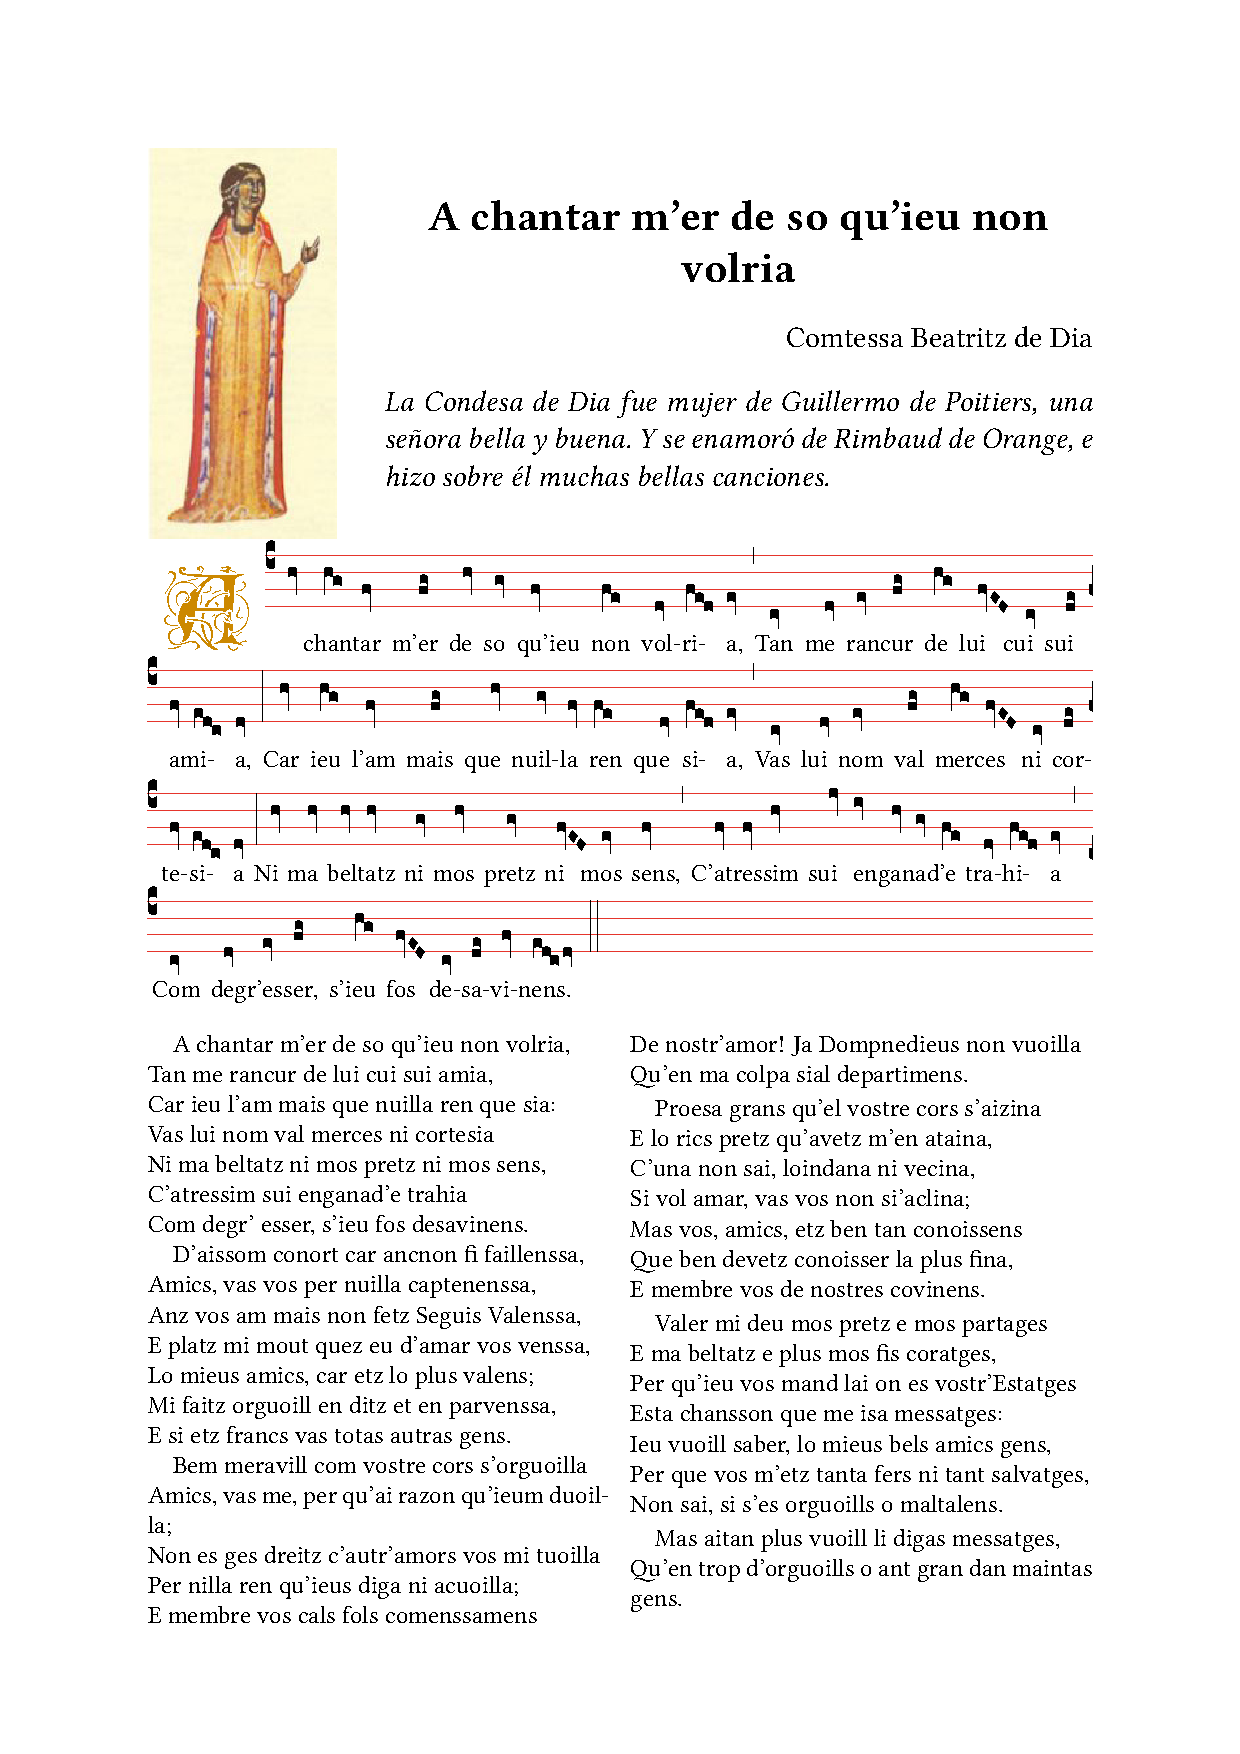
\includegraphics[width=1\linewidth]{figures/audicions/achantar} 

}

\end{figure}

\hypertarget{customisations-and-extensions}{%
\chapter{Customisations and extensions}\label{customisations-and-extensions}}

\minitoc 

\noindent This chapter describes a number of additional tips and tricks as well as possible customizations to the \texttt{oxforddown} thesis.

\hypertarget{front-matter}{%
\section{Front matter}\label{front-matter}}

\hypertarget{shorten-captions-shown-in-the-list-of-figures-pdf}{%
\subsection{Shorten captions shown in the list of figures (PDF)}\label{shorten-captions-shown-in-the-list-of-figures-pdf}}

You might want your list of figures (which follows the table of contents) to have shorter (or just different) figure descriptions than the actual figure captions.

Do this using the chunk option \texttt{fig.scap} (`short caption'), for example \texttt{\{r\ captain-image,\ fig.cap="A\ very\ long\ and\ descriptive\ (and\ potentially\ boring)\ caption\ that\ doesn\textquotesingle{}t\ fit\ in\ the\ list\ of\ figures,\ but\ helps\ the\ reader\ understand\ what\ the\ figure\ communicates.",\ fig.scap="A\ concise\ description\ for\ the\ list\ of\ figures"}

\hypertarget{shorten-captions-shown-in-the-list-of-tables-pdf}{%
\subsection{Shorten captions shown in the list of tables (PDF)}\label{shorten-captions-shown-in-the-list-of-tables-pdf}}

You might want your list of tables (which follows the list of figures in your thesis front matter) to have shorter (or just different) table descriptions than the actual table captions.

If you are using \texttt{knitr::kable} to generate a table, you can do this with the argument \texttt{caption.short}, e.g.:

\begin{Shaded}
\begin{Highlighting}[]
\NormalTok{knitr}\SpecialCharTok{::}\FunctionTok{kable}\NormalTok{(mtcars,}
              \AttributeTok{caption =} \StringTok{"A very long and descriptive (and potentially}
\StringTok{              boring) caption that doesn\textquotesingle{}t fit in the list of figures,}
\StringTok{              but helps the reader understand what the figure }
\StringTok{              communicates."}\NormalTok{,}
              \AttributeTok{caption.short =} \StringTok{"A concise description for the list of tables"}\NormalTok{)}
\end{Highlighting}
\end{Shaded}

\hypertarget{shorten-running-header-pdf}{%
\section{Shorten running header (PDF)}\label{shorten-running-header-pdf}}

You might want a chapter's running header (i.e.~the header showing the title of the current chapter at the top of page) to be shorter (or just different) to the actual chapter title.

Do this by adding the latex command \texttt{\textbackslash{}chaptermark\{My\ shorter\ version\}} after your chapter title.

For example, chapter \ref{cites-and-refs}`s running header is simply 'Cites and cross-refs', because it begins like this:

\begin{Shaded}
\begin{Highlighting}[]
\FunctionTok{\# Citations, cross{-}references, and collaboration \{\#cites{-}and{-}refs\} }
\NormalTok{\textbackslash{}chaptermark\{Cites and cross{-}refs\}}
\end{Highlighting}
\end{Shaded}

\hypertarget{unnumbered-chapters}{%
\section{Unnumbered chapters}\label{unnumbered-chapters}}

To make chapters unnumbered (normally only relevant to the Introduction and/or the Conclusion), follow the chapter header with \texttt{\{-\}}, e.g.~\texttt{\#\ Introduction\ \{-\}}.

When you do this, you must also follow the heading with these two latex commands:

\begin{Shaded}
\begin{Highlighting}[]
\FunctionTok{\textbackslash{}adjustmtc}
\FunctionTok{\textbackslash{}markboth}\NormalTok{\{The Name of Your Unnumbered Chapter\}\{\}}
\end{Highlighting}
\end{Shaded}

Otherwise the chapter's mini table of contents and the running header will show the previous chapter.

\hypertarget{beginning-chapters-with-quotes-pdf}{%
\section{Beginning chapters with quotes (PDF)}\label{beginning-chapters-with-quotes-pdf}}

The OxThesis LaTeX template lets you inject some wittiness into your thesis by including a block of type \texttt{savequote} at the beginning of chapters.
To do this, use the syntax \texttt{\textasciigrave{}\textasciigrave{}\textasciigrave{}\{block\ type=\textquotesingle{}savequote\textquotesingle{}\}}.\footnote{For more on custom block types, see the relevant section in \href{https://bookdown.org/yihui/bookdown/custom-blocks.html}{\emph{Authoring Books with R Markdown}}.}

Add the reference for the quote with the chunk option \texttt{quote\_author="my\ author\ name"}.
You will also want to add the chunk option \texttt{include=knitr::is\_latex\_output()} so that quotes are only included in PDF output.

It's not possible to use markdown syntax inside chunk options, so if you want to e.g.~italicise a book name in the reference use a \href{https://bookdown.org/yihui/bookdown/markdown-extensions-by-bookdown.html\#text-references}{`text reference'}: Create a named piece of text with `(ref:label-name) My text', then point to this in the chunk option with \texttt{quote\_author=\textquotesingle{}(ref:label-name)\textquotesingle{}}.

\hypertarget{highlighting-corrections-html-pdf}{%
\section{Highlighting corrections (HTML \& PDF)}\label{highlighting-corrections-html-pdf}}

For when it comes time to do corrections, you may want to highlight changes made when you submit a post-viva, corrected copy to your examiners so they can quickly verify you've completed the task.
You can do so like this:

\hypertarget{short-inline-corrections}{%
\subsection{Short, inline corrections}\label{short-inline-corrections}}

Highlight \textbf{short, inline corrections} by doing \texttt{{[}like\ this{]}\{.correction\}} --- the text between the square brackets will then \hl{be highlighted in blue} in the output.

Note that pandoc might get confused by citations and cross-references inside inline corrections.
In particular, it might get confused by \texttt{"{[}what\ @Shea2014\ said{]}\{.correction\}"} which becomes \hl{what \textcite{Shea2014} said}
In such cases, you can use LaTeX syntax directly.
The correction highlighting uses the \href{https://ctan.org/pkg/soul}{soul} package, so you can do like this:

\begin{itemize}
\tightlist
\item
  If using biblatex for references, use \texttt{"\textbackslash{}hl\{what\ \textbackslash{}textcite\{Shea2014\}\ said\}}
\item
  If using natbib for references, use \texttt{"\textbackslash{}hl\{what\ \textbackslash{}cite\{Shea2014\}\ said\}}
\end{itemize}

Using raw LaTeX has the drawback of corrections then not showing up in HTML output at all, but you might only care about correction highlighting in the PDF for your examiners anyway!

\hypertarget{blocks-of-added-or-changed-material}{%
\subsection{Blocks of added or changed material}\label{blocks-of-added-or-changed-material}}

Highlight entire \textbf{blocks of added or changed material} by putting them in a block of type \texttt{correction}, using the syntax \texttt{\textasciigrave{}\textasciigrave{}\textasciigrave{}\{block\ type=\textquotesingle{}correction\textquotesingle{}\}}.\footnote{In the \textbf{.tex} file for PDF output, this will put the content between \texttt{\textbackslash{}begin\{correction\}} and \texttt{\textbackslash{}end\{correction\}}; in gitbook output it will be put between \texttt{\textless{}div\ class="correction"\textgreater{}} and \texttt{\textless{}/div\textgreater{}}.}
Like so:

\begin{correction}
For larger chunks, like this paragraph or indeed entire figures, you can
use the \texttt{correction} block type. This environment
\textbf{highlights paragraph-sized and larger blocks} with the same blue
colour.
\end{correction}

\emph{Note that correction blocks cannot be included in word output.}

\hypertarget{stopping-corrections-from-being-highlighted}{%
\subsection{Stopping corrections from being highlighted}\label{stopping-corrections-from-being-highlighted}}

To turn off correction highlighting, go to the YAML header of \textbf{index.Rmd}, then:

\begin{itemize}
\tightlist
\item
  PDF output: set \texttt{corrections:\ false}\\
\item
  HTML output: remove or comment out \texttt{-\ templates/corrections.css}
\end{itemize}

\hypertarget{apply-custom-font-color-and-highlighting-to-text-html-pdf}{%
\section{Apply custom font color and highlighting to text (HTML \& PDF)}\label{apply-custom-font-color-and-highlighting-to-text-html-pdf}}

The lua filter that adds the functionality to highlight corrections adds two more tricks:
you can apply your own choice of colour to highlight text, or change the font color.
The syntax is as follows:

\begin{quote}
Here's \texttt{{[}some\ text\ in\ pink\ highlighting{]}\{highlight="pink"\}}\\
Becomes: Here's \sethlcolor{pink}\hl{some text in pink highlighting}\sethlcolor{correctioncolor}.
\end{quote}

\begin{quote}
\texttt{{[}Here\textquotesingle{}s\ some\ text\ with\ blue\ font{]}\{color="blue"\}}\strut \\
Becomes: \textcolor{blue}{Here's some text with blue font}
\end{quote}

\begin{quote}
Finally --- never, ever actually do this -- \texttt{{[}here\textquotesingle{}s\ some\ text\ with\ black\ highlighting\ and\ yellow\ font{]}\{highlight="black"\ color="yellow"\}}\\
Becomes: \textcolor{yellow}{\sethlcolor{black}\hl{here's some text with black highlighting and yellow font}\sethlcolor{correctioncolor}}
\end{quote}

The file \textbf{scripts\_and\_filters/colour\_and\_highlight.lua} implements this, if you want to fiddle around with it.
It works with both PDF and HTML output.

\hypertarget{embed-pdf}{%
\section{Including another paper in your thesis - embed a PDF document}\label{embed-pdf}}

You may want to embed existing PDF documents into the thesis, for example if your department allows a `portfolio' style thesis and you need to include an existing typeset publication as a chapter.

In gitbook output, you can simply use \texttt{knitr::include\_graphics} and it should include a scrollable (and downloadable) PDF.
You will probably want to set the chunk options \texttt{out.width=\textquotesingle{}100\%\textquotesingle{}} and \texttt{out.height=\textquotesingle{}1000px\textquotesingle{}}:

\begin{Shaded}
\begin{Highlighting}[]
\NormalTok{knitr}\SpecialCharTok{::}\FunctionTok{include\_graphics}\NormalTok{(}\StringTok{"figures/sample{-}content/pdf\_embed\_example/Lyngs2020\_FB.pdf"}\NormalTok{)}
\end{Highlighting}
\end{Shaded}

In LaTeX output, however, this approach can cause odd behaviour.
Therefore, when you build your thesis to PDF, split the PDF into an alphanumerically sorted sequence of \textbf{single-page} PDF files (you can do this automatically with the package \texttt{pdftools}). You can then use the appropriate LaTeX command to insert them, as shown below (for brevity, in the \texttt{oxforddown} PDF sample content we're only including two pages).
\emph{Note that the chunk option \texttt{results=\textquotesingle{}asis\textquotesingle{}} must be set.}
You may also want to remove margins from the PDF files, which you can do with Adobe Acrobat (paid version) and likely other software.

\begin{Shaded}
\begin{Highlighting}[]
\CommentTok{\# install.packages(pdftools)}
\CommentTok{\# split PDF into pages stored in}
\NormalTok{    figures}\SpecialCharTok{/}\NormalTok{sample}\SpecialCharTok{{-}}\NormalTok{content}\SpecialCharTok{/}\NormalTok{pdf\_embed\_example}\SpecialCharTok{/}\NormalTok{split}\SpecialCharTok{/}
\CommentTok{\#}
\NormalTok{    pdftools}\SpecialCharTok{::}\FunctionTok{pdf\_split}\NormalTok{(}\StringTok{"figures/sample{-}content/pdf\_embed\_example/Lyngs2020\_FB.pdf"}\NormalTok{,}
\CommentTok{\# output = "figures/sample{-}content/pdf\_embed\_example/split/")}

\CommentTok{\# grab the pages}
\NormalTok{pages }\OtherTok{\textless{}{-}} \FunctionTok{list.files}\NormalTok{(}\StringTok{"figures/sample{-}content/pdf\_embed\_example/split"}\NormalTok{,}
    \AttributeTok{full.names =} \ConstantTok{TRUE}\NormalTok{)}

\CommentTok{\# set how wide you want the inserted PDFs to be:}
\CommentTok{\# 1.0 is 100 per cent of the oxforddown PDF page width;}
\CommentTok{\# you may want to make it a bit bigger}
\NormalTok{pdf\_width }\OtherTok{\textless{}{-}} \FloatTok{1.2}

\CommentTok{\# for each PDF page, insert it nicely and}
\CommentTok{\# end with a page break}
\FunctionTok{cat}\NormalTok{(stringr}\SpecialCharTok{::}\FunctionTok{str\_c}\NormalTok{(}\StringTok{"}\SpecialCharTok{\textbackslash{}\textbackslash{}}\StringTok{newpage }\SpecialCharTok{\textbackslash{}\textbackslash{}}\StringTok{begin\{center\}}
\StringTok{    }\SpecialCharTok{\textbackslash{}\textbackslash{}}\StringTok{makebox[}\SpecialCharTok{\textbackslash{}\textbackslash{}}\StringTok{linewidth][c]\{}\SpecialCharTok{\textbackslash{}\textbackslash{}}\StringTok{includegraphics[width="}\NormalTok{, pdf\_width,}
    \StringTok{"}\SpecialCharTok{\textbackslash{}\textbackslash{}}\StringTok{linewidth]\{"}\NormalTok{, pages, }\StringTok{"\}\} }\SpecialCharTok{\textbackslash{}\textbackslash{}}\StringTok{end\{center\}"}\NormalTok{))}
\end{Highlighting}
\end{Shaded}

\newpage \begin{center} \makebox[\linewidth][c]{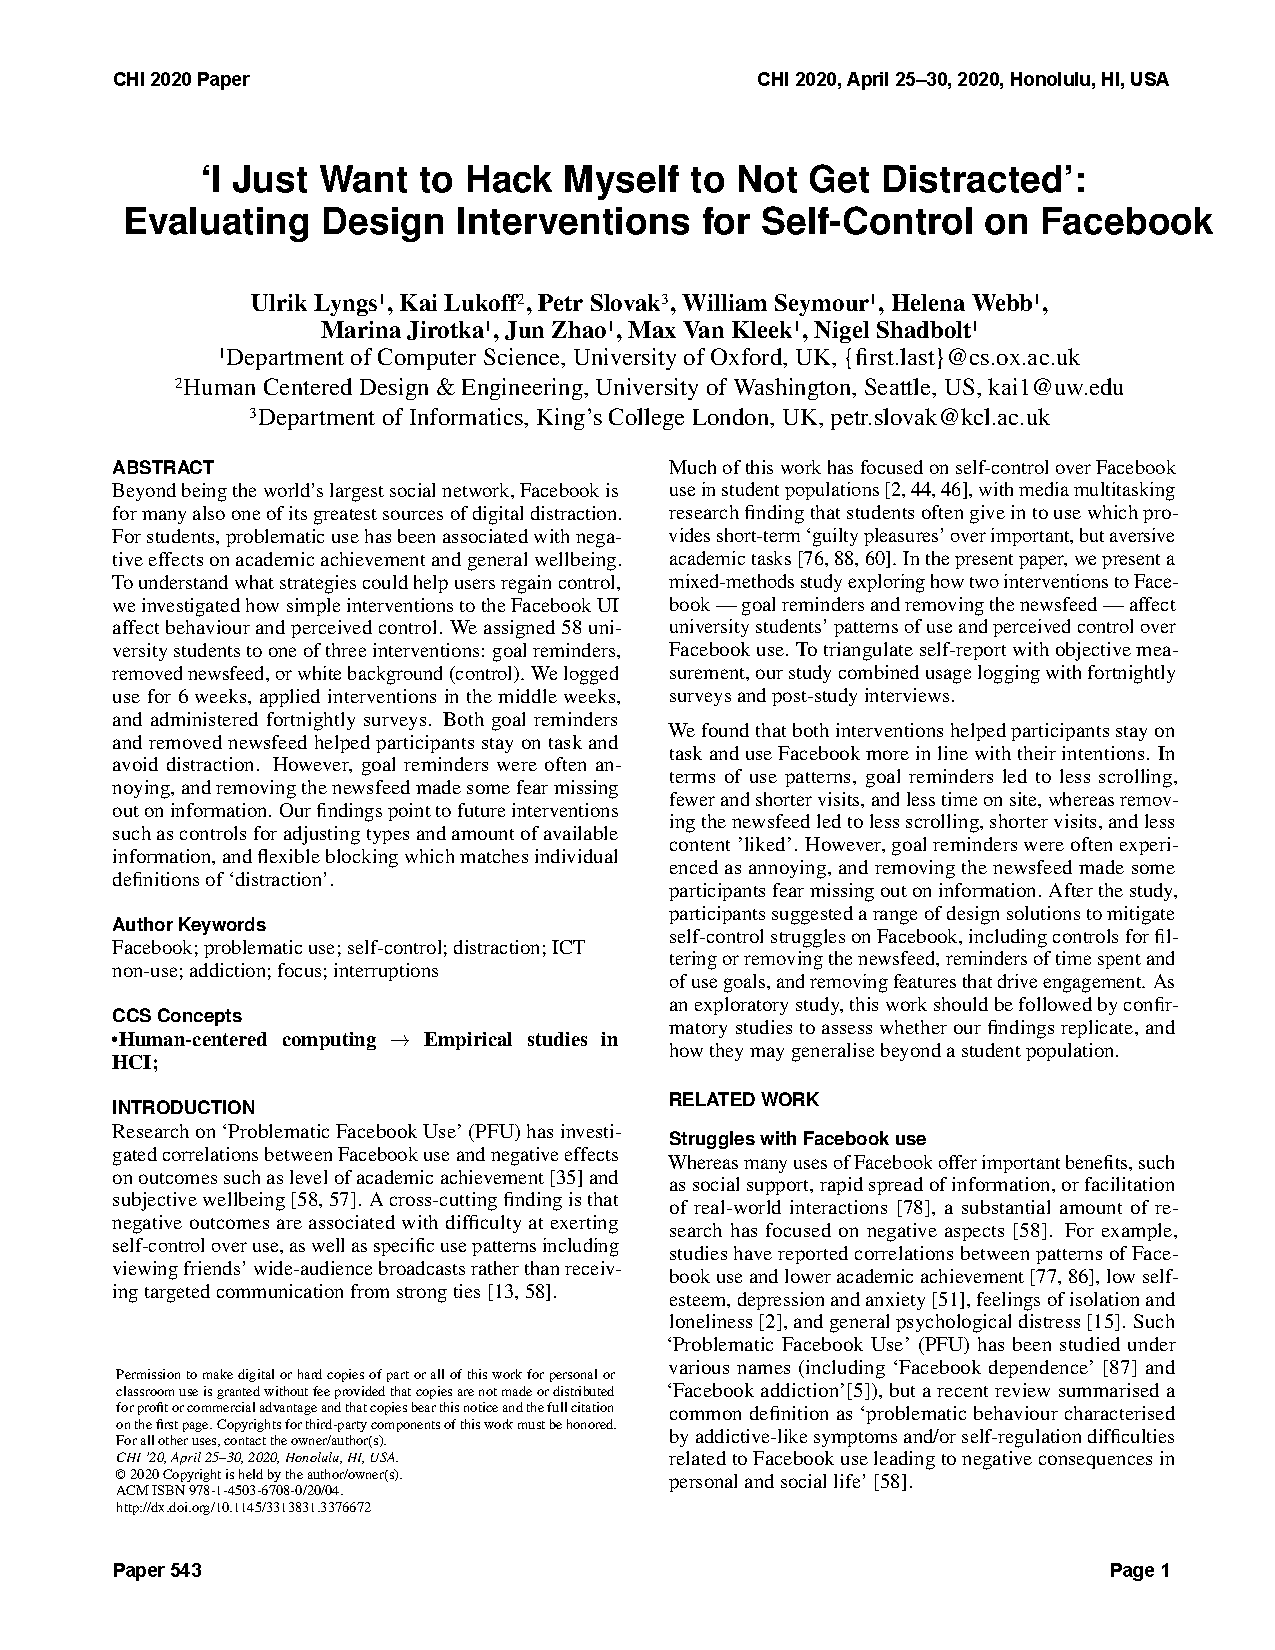
\includegraphics[width=1.2\linewidth]{figures/sample-content/pdf_embed_example/split/_000000000000001.pdf}} \end{center} \newpage \begin{center} \makebox[\linewidth][c]{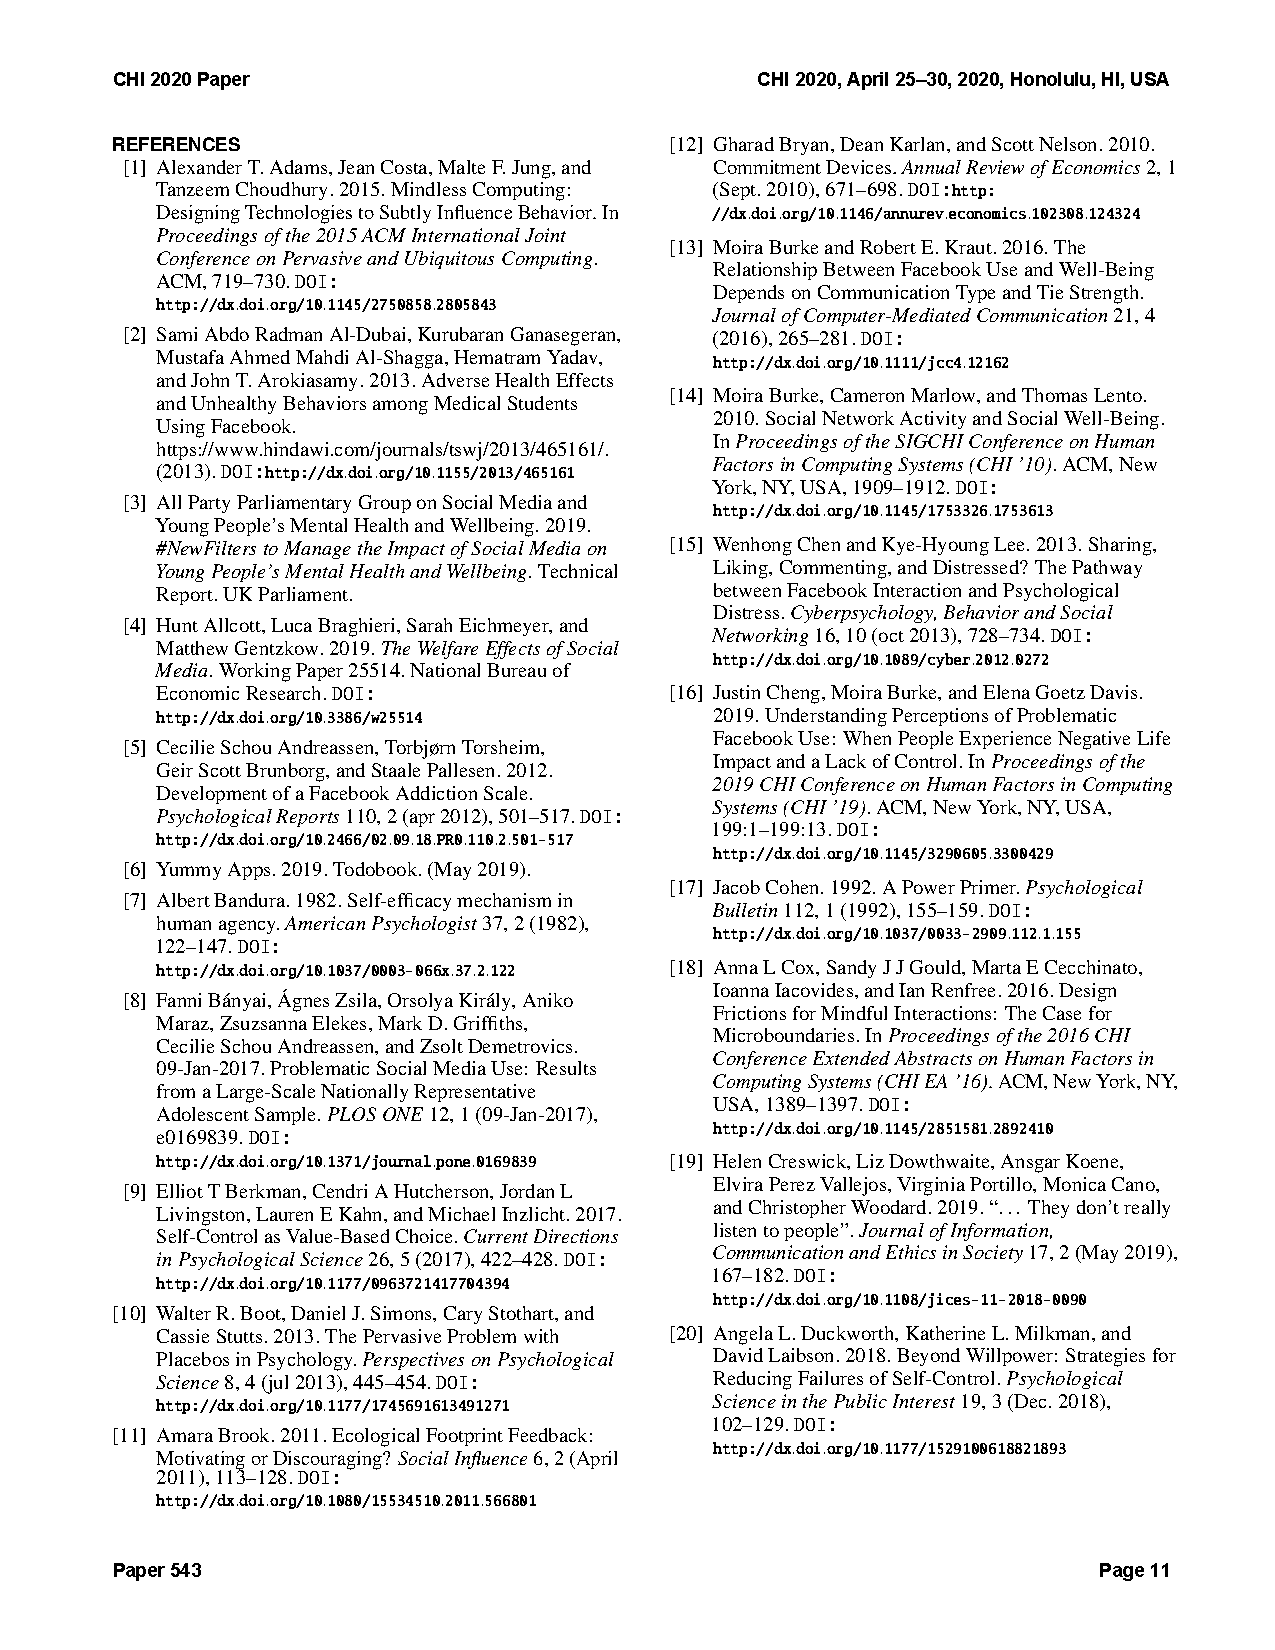
\includegraphics[width=1.2\linewidth]{figures/sample-content/pdf_embed_example/split/_000000000000011.pdf}} \end{center}

\hypertarget{embed-rmd}{%
\section{Including another paper in your thesis - R Markdown child document}\label{embed-rmd}}

Sometimes you want to include another paper you are currently writing as a chapter in your thesis.
Above \ref{embed-pdf}, we described the simplest way to do this: include the other paper as a pdf.
However, in some cases you instead want to include the R Markdown source from this paper, and have it compiled within your thesis.
This is a little bit more tricky, because you need to keep careful track of your file paths, but it is possible by \href{https://bookdown.org/yihui/rmarkdown-cookbook/child-document.html}{including the paper as a child document}.
There are four main steps:

\begin{enumerate}
\def\labelenumi{\arabic{enumi}.}
\tightlist
\item
  Include the paper as a child document
\item
  Make file paths compatible with knitting the article on its own, as well as when it's include in your thesis
\item
  Make header levels correct
\item
  Make figure widths correct
\end{enumerate}

\hypertarget{an-example-paper-in-another-folder}{%
\subsection{An example paper in another folder}\label{an-example-paper-in-another-folder}}

Take this simple example (files for this are in \href{https://github.com/ulyngs/oxforddown-external-article}{this GitHub repository}):

\begin{Shaded}
\begin{Highlighting}[]
\NormalTok{|{-}{-}paper\_to\_include}
\NormalTok{|  |{-}{-}my\_paper.Rmd}
\NormalTok{|  |{-}{-}data}
\NormalTok{|  |  |{-}{-}cat\_salt.csv}
\NormalTok{|  |{-}{-}figures}
\NormalTok{|  |  |{-}{-}cat.jpg}
\NormalTok{|}
\NormalTok{|{-}{-}thesis}
\end{Highlighting}
\end{Shaded}

As the chart suggests, you have another folder, \textbf{paper\_to\_include/} living in the same containing folder as your thesis folder.
In the \textbf{paper\_to\_include} folder, the file \textbf{my\_paper.Rmd} is where you write the paper.
In \textbf{my\_paper.Rmd}, you read in a CSV file found in the subfolder \textbf{data/cats.csv}, and also an image from the subfolder \textbf{figures/cat.jpg}.

\hypertarget{step-1-include-paper-as-a-child-document}{%
\subsection{Step 1: Include paper as a child document}\label{step-1-include-paper-as-a-child-document}}

In your thesis folder, create an Rmd file for the chapter where you want to include another paper.
Add one or more code chunks that include R Markdown files from that paper as child documents:

\begin{Shaded}
\begin{Highlighting}[]
\FunctionTok{\# Including an external chapter }

\InformationTok{\textasciigrave{}\textasciigrave{}\textasciigrave{}\{r child = "../paper\_to\_include/my\_paper.Rmd"\}}
\InformationTok{\textasciigrave{}\textasciigrave{}\textasciigrave{}}
\end{Highlighting}
\end{Shaded}

\hypertarget{step-2-make-file-paths-compatible}{%
\subsection{Step 2: Make file paths compatible}\label{step-2-make-file-paths-compatible}}

Use \href{https://rmarkdown.rstudio.com/lesson-6.html}{parameters} to adjust the file path of images based on values you set in the YAML header of an R Markdown file.
In \textbf{my\_paper.Rmd}, create a parameter called \texttt{other\_path} and set it to an empty string:

\begin{Shaded}
\begin{Highlighting}[]
\PreprocessorTok{{-}{-}{-}}
\FunctionTok{title}\KeywordTok{:}\AttributeTok{ }\StringTok{"A fabulous article in a different folder"}
\FunctionTok{params}\KeywordTok{:}
\AttributeTok{  }\FunctionTok{other\_path}\KeywordTok{:}\AttributeTok{ }\StringTok{""}
\PreprocessorTok{{-}{-}{-}}
\end{Highlighting}
\end{Shaded}

In \textbf{my\_paper.Rmd}, put this at the start of the filepath when you read in data or include images:

\begin{Shaded}
\begin{Highlighting}[]
\FunctionTok{library}\NormalTok{(tidyverse)}
\FunctionTok{library}\NormalTok{(knitr)}

\NormalTok{cat\_data }\OtherTok{\textless{}{-}} \FunctionTok{read\_csv}\NormalTok{(}\FunctionTok{str\_c}\NormalTok{(params}\SpecialCharTok{$}\NormalTok{other\_path, }\StringTok{"data/cats.csv"}\NormalTok{))}
\FunctionTok{include\_graphics}\NormalTok{(}\FunctionTok{str\_c}\NormalTok{(params}\SpecialCharTok{$}\NormalTok{other\_path, }\StringTok{"figures/cat.jpg"}\NormalTok{))}
\end{Highlighting}
\end{Shaded}

Finally, in your thesis folder's \textbf{index.Rmd} file, also create the parameter \texttt{other\_path}.
But here, set it to where the \textbf{paper\_to\_include/} folder is relative to your thesis folder:

\begin{Shaded}
\begin{Highlighting}[]
\FunctionTok{params}\KeywordTok{:}
\AttributeTok{  }\FunctionTok{other\_path}\KeywordTok{:}\AttributeTok{ }\StringTok{"../paper\_to\_include/"}
\end{Highlighting}
\end{Shaded}

\hypertarget{note-on-html-output}{%
\subsubsection{Note on HTML output}\label{note-on-html-output}}

Note that if you want to host an HTML version on your thesis online, you will need to include graphics in the content that you host online - the internet obviously won't be able to see filepaths that are just referring to stuff in another folder on your computer!

\hypertarget{step-3-make-sure-header-levels-are-correct}{%
\subsection{Step 3: Make sure header levels are correct}\label{step-3-make-sure-header-levels-are-correct}}

Unless the paper you want to include is also written as a book, your header levels are probably going to be off.
That is, the level 1 headers (\# Some header) you use for main sections in the other paper turns into chaper titles when included in your thesis.

To avoid this, first \emph{increment all heading levels by one in \textbf{paper\_to\_include/my\_paper.Rmd}} (\# Some header -\textgreater{} \#\# Some header).
Then in \textbf{paper\_to\_include/} create a \href{https://bookdown.org/yihui/rmarkdown-cookbook/lua-filters.html\#lua-filters}{lua filter} that decrements header levels by one: Create a text file, save it as \textbf{reduce\_header\_level.lua}, and give it the content below.

\begin{Shaded}
\begin{Highlighting}[]
\KeywordTok{function}\NormalTok{ Header}\OperatorTok{(}\NormalTok{el}\OperatorTok{)}
  \ControlFlowTok{if} \OperatorTok{(}\NormalTok{el}\OperatorTok{.}\NormalTok{level }\OperatorTok{\textless{}=} \DecValTok{1}\OperatorTok{)} \ControlFlowTok{then}
    \FunctionTok{error}\OperatorTok{(}\StringTok{"I don\textquotesingle{}t know how to decrease the level of h1"}\OperatorTok{)}
  \ControlFlowTok{end}
\NormalTok{  el}\OperatorTok{.}\NormalTok{level }\OperatorTok{=}\NormalTok{ el}\OperatorTok{.}\NormalTok{level }\OperatorTok{{-}} \DecValTok{1}
  \ControlFlowTok{return}\NormalTok{ el}
\KeywordTok{end}
\end{Highlighting}
\end{Shaded}

In the YAML header of \textbf{paper\_to\_include/my\_paper.Rmd}, use this filter:

\begin{Shaded}
\begin{Highlighting}[]
\PreprocessorTok{{-}{-}{-}}
\FunctionTok{title}\KeywordTok{:}\AttributeTok{ }\StringTok{"A fabulous article in a different folder"}
\FunctionTok{params}\KeywordTok{:}
\AttributeTok{  }\FunctionTok{other\_path}\KeywordTok{:}\AttributeTok{ }\StringTok{""}
\FunctionTok{output}\KeywordTok{:}
\AttributeTok{  }\FunctionTok{pdf\_document}\KeywordTok{:}\AttributeTok{ }
\AttributeTok{    }\FunctionTok{pandoc\_args}\KeywordTok{:}\AttributeTok{ }\KeywordTok{[}\StringTok{"{-}{-}lua{-}filter=reduce\_header\_level.lua"}\KeywordTok{]}
\PreprocessorTok{{-}{-}{-}}
\end{Highlighting}
\end{Shaded}

Now, your header levels will be correct both when you knit the paper on its own and when its included in your thesis.

NOTE: There might be no need to use a lua filter to shift heading - it seems you could simply use \texttt{pandoc\_args:\ {[}"-\/-shift-heading-level-by=-1"{]}} (see \url{https://pandoc.org/MANUAL.html\#reader-options})

\hypertarget{step-4.-make-sure-figure-widths-are-correct}{%
\subsection{Step 4. Make sure figure widths are correct}\label{step-4.-make-sure-figure-widths-are-correct}}

It might be that your figure widths when knitting your paper on its own, and when including it in your thesis, need to be different.
You can again use parameters to set figure widths.

Imagine you want figure width to be 80\% of the page width when knitting your paper on its own, but 100\% in your thesis.
In \textbf{paper\_to\_include/my\_paper.Rmd}, first add a parameter we could call \texttt{out\_width} and set it to the string ``80\%'':

\begin{Shaded}
\begin{Highlighting}[]
\PreprocessorTok{{-}{-}{-}}
\FunctionTok{title}\KeywordTok{:}\AttributeTok{ }\StringTok{"A fabulous article in a different folder"}
\FunctionTok{params}\KeywordTok{:}
\AttributeTok{  }\FunctionTok{other\_path}\KeywordTok{:}\AttributeTok{ }\StringTok{""}
\AttributeTok{  }\FunctionTok{out\_width}\KeywordTok{:}\AttributeTok{ }\StringTok{"80\%"}
\FunctionTok{output}\KeywordTok{:}
\AttributeTok{  }\FunctionTok{pdf\_document}\KeywordTok{:}\AttributeTok{ }
\AttributeTok{    }\FunctionTok{pandoc\_args}\KeywordTok{:}\AttributeTok{ }\KeywordTok{[}\StringTok{"{-}{-}lua{-}filter=reduce\_header\_level.lua"}\KeywordTok{]}
\PreprocessorTok{{-}{-}{-}}
\end{Highlighting}
\end{Shaded}

Then, make sure use that parameter to set the output width when you include figures in \textbf{paper\_to\_include/my\_paper.Rmd}:

\begin{Shaded}
\begin{Highlighting}[]
\InformationTok{\textasciigrave{}\textasciigrave{}\textasciigrave{}\{r, out.width=params$out\_width, fig.cap="A very funny cat"\}}
\InformationTok{include\_graphics(str\_c(params$other\_path, "figures/cat.jpg"))}
\InformationTok{\textasciigrave{}\textasciigrave{}\textasciigrave{}}
\end{Highlighting}
\end{Shaded}

Finally, create the parameter \texttt{out\_width} in your thesis' \textbf{index.Rmd} file:

\begin{Shaded}
\begin{Highlighting}[]
\FunctionTok{params}\KeywordTok{:}
\AttributeTok{  }\FunctionTok{other\_path}\KeywordTok{:}\AttributeTok{ }\StringTok{"../paper\_to\_include/"}
\AttributeTok{  }\FunctionTok{out\_width}\KeywordTok{:}\AttributeTok{ }\StringTok{"80\%"}
\end{Highlighting}
\end{Shaded}

Now, the output width of your figure will be 80\% when knitting your paper on its own, and 100\% when knitting it as child document of your thesis.

\hypertarget{customizing-referencing}{%
\section{Customizing referencing}\label{customizing-referencing}}

\hypertarget{using-a-.csl-file-with-pandoc-instead-of-biblatex}{%
\subsection{Using a .csl file with pandoc instead of biblatex}\label{using-a-.csl-file-with-pandoc-instead-of-biblatex}}

The \texttt{oxforddown} package uses biblatex in LaTeX for referencing.
It is also possible to use pandoc for referencing by providing a .csl file in the YAML header of \textbf{index.Rmd} (likely requiring commenting out the biblatex code in \textbf{templates/template.tex}).
This may be helpful for those who have a .csl file describing the referencing format for a particular journal.
However, note that this approach does not support chapter bibliographies (see Section \ref{biblatex-custom}).

\begin{Shaded}
\begin{Highlighting}[]
\FunctionTok{csl}\KeywordTok{:}\AttributeTok{ ecology.csl}
\end{Highlighting}
\end{Shaded}

\hypertarget{biblatex-custom}{%
\subsection{Customizing biblatex and adding chapter bibliographies}\label{biblatex-custom}}

This section provides one example of customizing biblatex. Much of this code was combined from searches on Stack Exchange and other sources (e.g.~\href{https://tex.stackexchange.com/questions/10682/suppress-in-biblatex}{here}).

In \textbf{templates/template.tex}, one can replace the existing biblatex calls with the following to achieve referencing that looks like this:

(Charmantier and Gienapp 2014)

Charmantier, A. and P. Gienapp (2014). Climate change and timing of avian breeding and migration: evolutionary versus plastic changes. Evolutionary Applications 7(1):15--28. doi: 10.1111/eva.12126.

\begin{Shaded}
\begin{Highlighting}[]
\BuiltInTok{\textbackslash{}usepackage}\NormalTok{[backend=biber,}
\NormalTok{    bibencoding=utf8,}
\NormalTok{    refsection=chapter, }\CommentTok{\% referencing by chapter}
\NormalTok{    style=authoryear, }
\NormalTok{    firstinits=true,}
\NormalTok{    isbn=false,}
\NormalTok{    doi=true,}
\NormalTok{    url=false,}
\NormalTok{    eprint=false,}
\NormalTok{    related=false,}
\NormalTok{    dashed=false,}
\NormalTok{    clearlang=true,}
\NormalTok{    maxcitenames=2,}
\NormalTok{    mincitenames=1,}
\NormalTok{    maxbibnames=10,}
\NormalTok{    abbreviate=false,}
\NormalTok{    minbibnames=3,}
\NormalTok{    uniquelist=minyear,}
\NormalTok{    sortcites=true,}
\NormalTok{    date=year}
\NormalTok{]\{}\ExtensionTok{biblatex}\NormalTok{\}}
\FunctionTok{\textbackslash{}AtEveryBibitem}\NormalTok{\{}\CommentTok{\%}
  \FunctionTok{\textbackslash{}clearlist}\NormalTok{\{language\}}\CommentTok{\%}
  \FunctionTok{\textbackslash{}clearfield}\NormalTok{\{note\}}
\NormalTok{\}}

\FunctionTok{\textbackslash{}DeclareFieldFormat}\NormalTok{\{titlecase\}\{}\FunctionTok{\textbackslash{}MakeTitleCase}\NormalTok{\{\#1\}\}}

\FunctionTok{\textbackslash{}newrobustcmd}\NormalTok{\{}\FunctionTok{\textbackslash{}MakeTitleCase}\NormalTok{\}[1]\{}\CommentTok{\%}
  \FunctionTok{\textbackslash{}ifthenelse}\NormalTok{\{}\FunctionTok{\textbackslash{}ifcurrentfield}\NormalTok{\{booktitle\}}\FunctionTok{\textbackslash{}OR\textbackslash{}ifcurrentfield}\NormalTok{\{booksubtitle\}}\CommentTok{\%}
    \FunctionTok{\textbackslash{}OR\textbackslash{}ifcurrentfield}\NormalTok{\{maintitle\}}\FunctionTok{\textbackslash{}OR\textbackslash{}ifcurrentfield}\NormalTok{\{mainsubtitle\}}\CommentTok{\%}
    \FunctionTok{\textbackslash{}OR\textbackslash{}ifcurrentfield}\NormalTok{\{journaltitle\}}\FunctionTok{\textbackslash{}OR\textbackslash{}ifcurrentfield}\NormalTok{\{journalsubtitle\}}\CommentTok{\%}
    \FunctionTok{\textbackslash{}OR\textbackslash{}ifcurrentfield}\NormalTok{\{issuetitle\}}\FunctionTok{\textbackslash{}OR\textbackslash{}ifcurrentfield}\NormalTok{\{issuesubtitle\}}\CommentTok{\%}
    \FunctionTok{\textbackslash{}OR\textbackslash{}ifentrytype}\NormalTok{\{book\}}\FunctionTok{\textbackslash{}OR\textbackslash{}ifentrytype}\NormalTok{\{mvbook\}}\FunctionTok{\textbackslash{}OR\textbackslash{}ifentrytype}\NormalTok{\{bookinbook\}}\CommentTok{\%}
    \FunctionTok{\textbackslash{}OR\textbackslash{}ifentrytype}\NormalTok{\{booklet\}}\FunctionTok{\textbackslash{}OR\textbackslash{}ifentrytype}\NormalTok{\{suppbook\}}\CommentTok{\%}
    \FunctionTok{\textbackslash{}OR\textbackslash{}ifentrytype}\NormalTok{\{collection\}}\FunctionTok{\textbackslash{}OR\textbackslash{}ifentrytype}\NormalTok{\{mvcollection\}}\CommentTok{\%}
    \FunctionTok{\textbackslash{}OR\textbackslash{}ifentrytype}\NormalTok{\{suppcollection\}}\FunctionTok{\textbackslash{}OR\textbackslash{}ifentrytype}\NormalTok{\{manual\}}\CommentTok{\%}
    \FunctionTok{\textbackslash{}OR\textbackslash{}ifentrytype}\NormalTok{\{periodical\}}\FunctionTok{\textbackslash{}OR\textbackslash{}ifentrytype}\NormalTok{\{suppperiodical\}}\CommentTok{\%}
    \FunctionTok{\textbackslash{}OR\textbackslash{}ifentrytype}\NormalTok{\{proceedings\}}\FunctionTok{\textbackslash{}OR\textbackslash{}ifentrytype}\NormalTok{\{mvproceedings\}}\CommentTok{\%}
    \FunctionTok{\textbackslash{}OR\textbackslash{}ifentrytype}\NormalTok{\{reference\}}\FunctionTok{\textbackslash{}OR\textbackslash{}ifentrytype}\NormalTok{\{mvreference\}}\CommentTok{\%}
    \FunctionTok{\textbackslash{}OR\textbackslash{}ifentrytype}\NormalTok{\{report\}}\FunctionTok{\textbackslash{}OR\textbackslash{}ifentrytype}\NormalTok{\{thesis\}\}}
\NormalTok{    \{\#1\}}
\NormalTok{    \{}\FunctionTok{\textbackslash{}MakeSentenceCase}\NormalTok{\{\#1\}\}\}}
    
\CommentTok{\% \textbackslash{}renewbibmacro\{in:\}\{\}}
\CommentTok{\% suppress "in" for articles}
\CommentTok{\% }
\FunctionTok{\textbackslash{}renewbibmacro}\NormalTok{\{in:\}\{}\CommentTok{\%}
  \FunctionTok{\textbackslash{}ifentrytype}\NormalTok{\{article\}\{\}\{}\FunctionTok{\textbackslash{}printtext}\NormalTok{\{}\FunctionTok{\textbackslash{}bibstring}\NormalTok{\{in\}}\FunctionTok{\textbackslash{}intitlepunct}\NormalTok{\}\}\}}
\CommentTok{\%{-}{-} no "quotes" around titles of chapters/article titles}
\FunctionTok{\textbackslash{}DeclareFieldFormat}\NormalTok{[article, inbook, incollection, inproceedings, misc, thesis, unpublished]}
\NormalTok{\{title\}\{\#1\}}
\CommentTok{\%{-}{-} no punctuation after volume}
\FunctionTok{\textbackslash{}DeclareFieldFormat}\NormalTok{[article]}
\NormalTok{\{volume\}\{\{\#1\}\}}
\CommentTok{\%{-}{-} puts number/issue between brackets}
\FunctionTok{\textbackslash{}DeclareFieldFormat}\NormalTok{[article, inbook, incollection, inproceedings, misc, thesis, unpublished]}
\NormalTok{\{number\}\{}\FunctionTok{\textbackslash{}mkbibparens}\NormalTok{\{\#1\}\} }
\CommentTok{\%{-}{-} and then for articles directly the pages w/o any "pages" or "pp." }
\FunctionTok{\textbackslash{}DeclareFieldFormat}\NormalTok{[article]}
\NormalTok{\{pages\}\{\#1\}}
\CommentTok{\%{-}{-} for some types replace "pages" by "p."}
\FunctionTok{\textbackslash{}DeclareFieldFormat}\NormalTok{[inproceedings, incollection, inbook]}
\NormalTok{\{pages\}\{p. \#1\}}
\CommentTok{\%{-}{-} format 16(4):224{-}{-}225 for articles}
\FunctionTok{\textbackslash{}renewbibmacro*}\NormalTok{\{volume+number+eid\}\{}
  \FunctionTok{\textbackslash{}printfield}\NormalTok{\{volume\}}\CommentTok{\%}
  \FunctionTok{\textbackslash{}printfield}\NormalTok{\{number\}}\CommentTok{\%}
  \FunctionTok{\textbackslash{}printunit}\NormalTok{\{}\FunctionTok{\textbackslash{}addcolon}\NormalTok{\}}
\NormalTok{\}}
\end{Highlighting}
\end{Shaded}

If you would like chapter bibliographies, in addition insert the following code at the end of each chapter, and comment out the entire REFERENCES section at the end of template.tex.

\begin{Shaded}
\begin{Highlighting}[]
\FunctionTok{\textbackslash{}printbibliography}\NormalTok{[segment=}\FunctionTok{\textbackslash{}therefsection}\NormalTok{,heading=subbibliography]}
\end{Highlighting}
\end{Shaded}

\hypertarget{customizing-the-page-headers-and-footers-pdf}{%
\section{Customizing the page headers and footers (PDF)}\label{customizing-the-page-headers-and-footers-pdf}}

This can now be done directly in \textbf{index.Rmd}'s YAML header.
If you are a LaTeX expert and need further customisation that what's currently provided, you can tweak the relevant sections of \textbf{templates/template.tex} - the relevant code is beneath the line that begins \texttt{\textbackslash{}usepackage\{fancyhdr\}}.

\hypertarget{diving-in-to-the-oxthesis-latex-template-pdf}{%
\section{Diving in to the OxThesis LaTeX template (PDF)}\label{diving-in-to-the-oxthesis-latex-template-pdf}}

For LaTeX minded people, you can read through \textbf{templates/template.tex} to see which additional customisation options are available as well as \textbf{templates/ociamthesis.cls} which supplies the base class.
For example, \textbf{template.tex} provides an option for master's degree submissions, which changes identifying information to candidate number and includes a word count.
At the time of writing, you must set this directly in \textbf{template.tex} rather than from the YAML header in \textbf{index.Rmd}.

\hypertarget{customising-to-a-different-university}{%
\section{Customising to a different university}\label{customising-to-a-different-university}}

\hypertarget{the-minimal-route}{%
\subsection{The minimal route}\label{the-minimal-route}}

If the front matter in the OxThesis LaTeX template is suitable to your university, customising \texttt{oxforddown} to your needs could be as simple as putting the name of your institution and the path to your university's logo in \textbf{index.Rmd}:

\begin{Shaded}
\begin{Highlighting}[]
\FunctionTok{university}\KeywordTok{:}\AttributeTok{ University of You}
\FunctionTok{university{-}logo}\KeywordTok{:}\AttributeTok{ figures/your{-}logo{-}here.pdf}
\end{Highlighting}
\end{Shaded}

\hypertarget{replacing-the-entire-title-page-with-your-required-content}{%
\subsection{Replacing the entire title page with your required content}\label{replacing-the-entire-title-page-with-your-required-content}}

If you have a \textbf{.tex} file with some required front matter from your university that you want to replace the OxThesis template's title page altogether, you can provide a filepath to this file in \textbf{index.Rmd}.
\texttt{oxforddown}'s sample content includes and example of this --- if you use the YAML below, your front matter will look like this:

\begin{Shaded}
\begin{Highlighting}[]
\FunctionTok{alternative{-}title{-}page}\KeywordTok{:}\AttributeTok{ front{-}and{-}back{-}matter/alt{-}title{-}page{-}example.tex}
\end{Highlighting}
\end{Shaded}

\noindent
\fbox{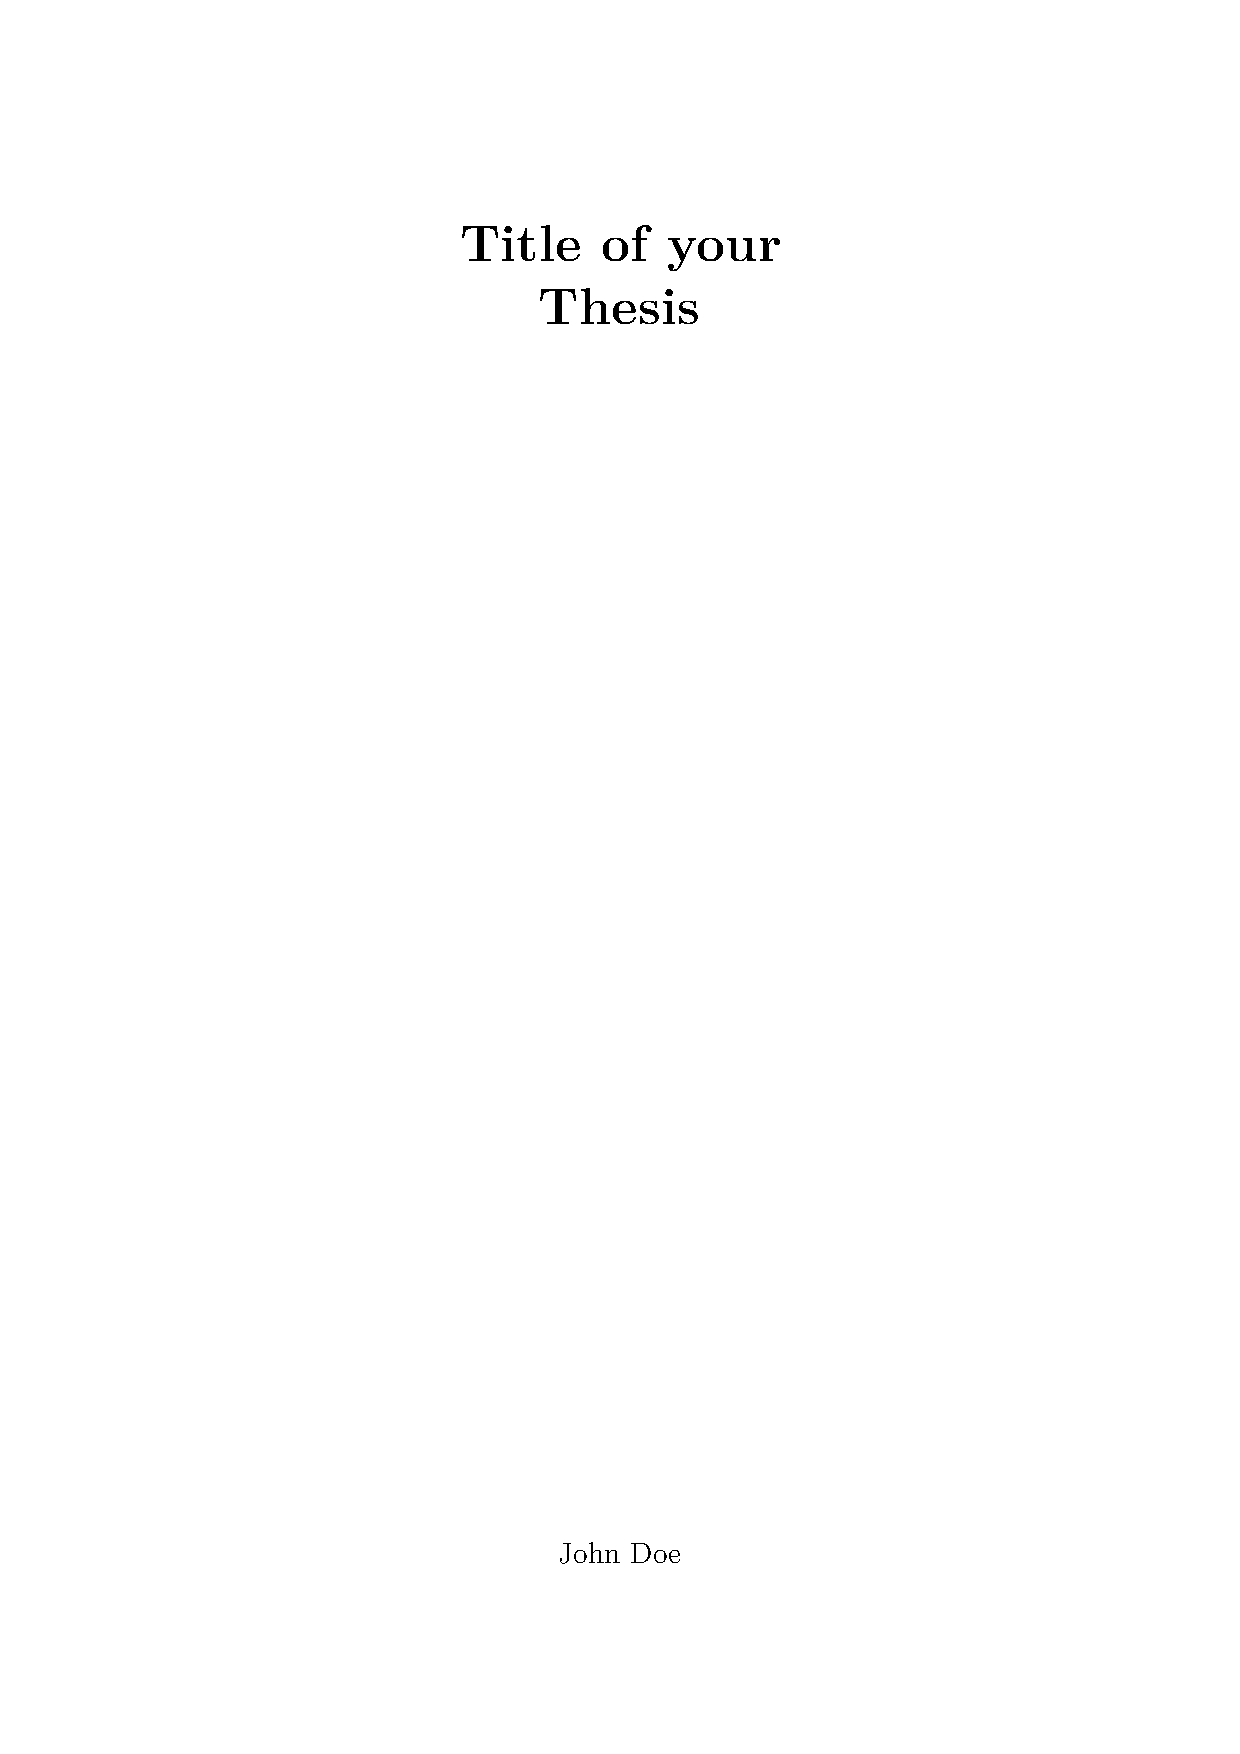
\includegraphics[width=0.32\linewidth]{figures/sample-content/alt_frontmatter_example/split/_000001.pdf}} \fbox{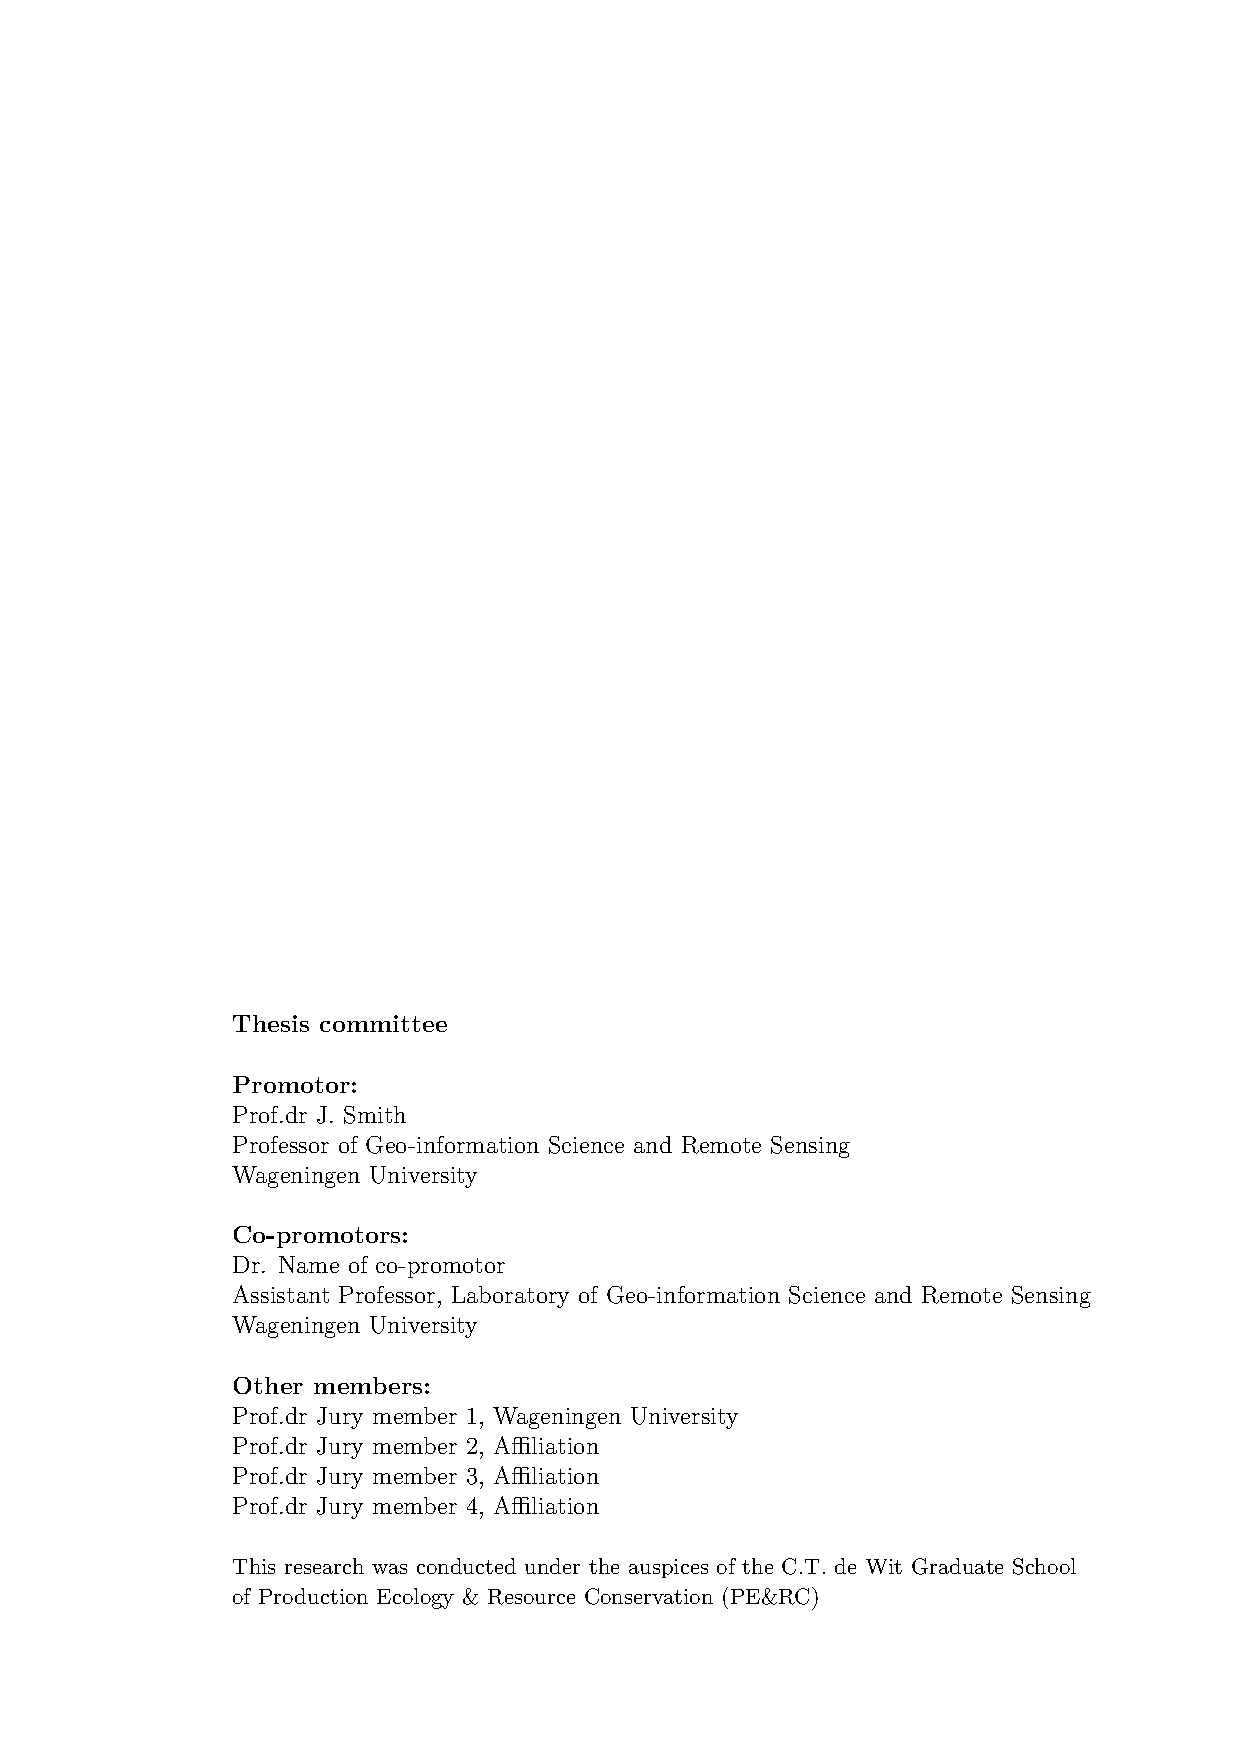
\includegraphics[width=0.32\linewidth]{figures/sample-content/alt_frontmatter_example/split/_000002.pdf}} \fbox{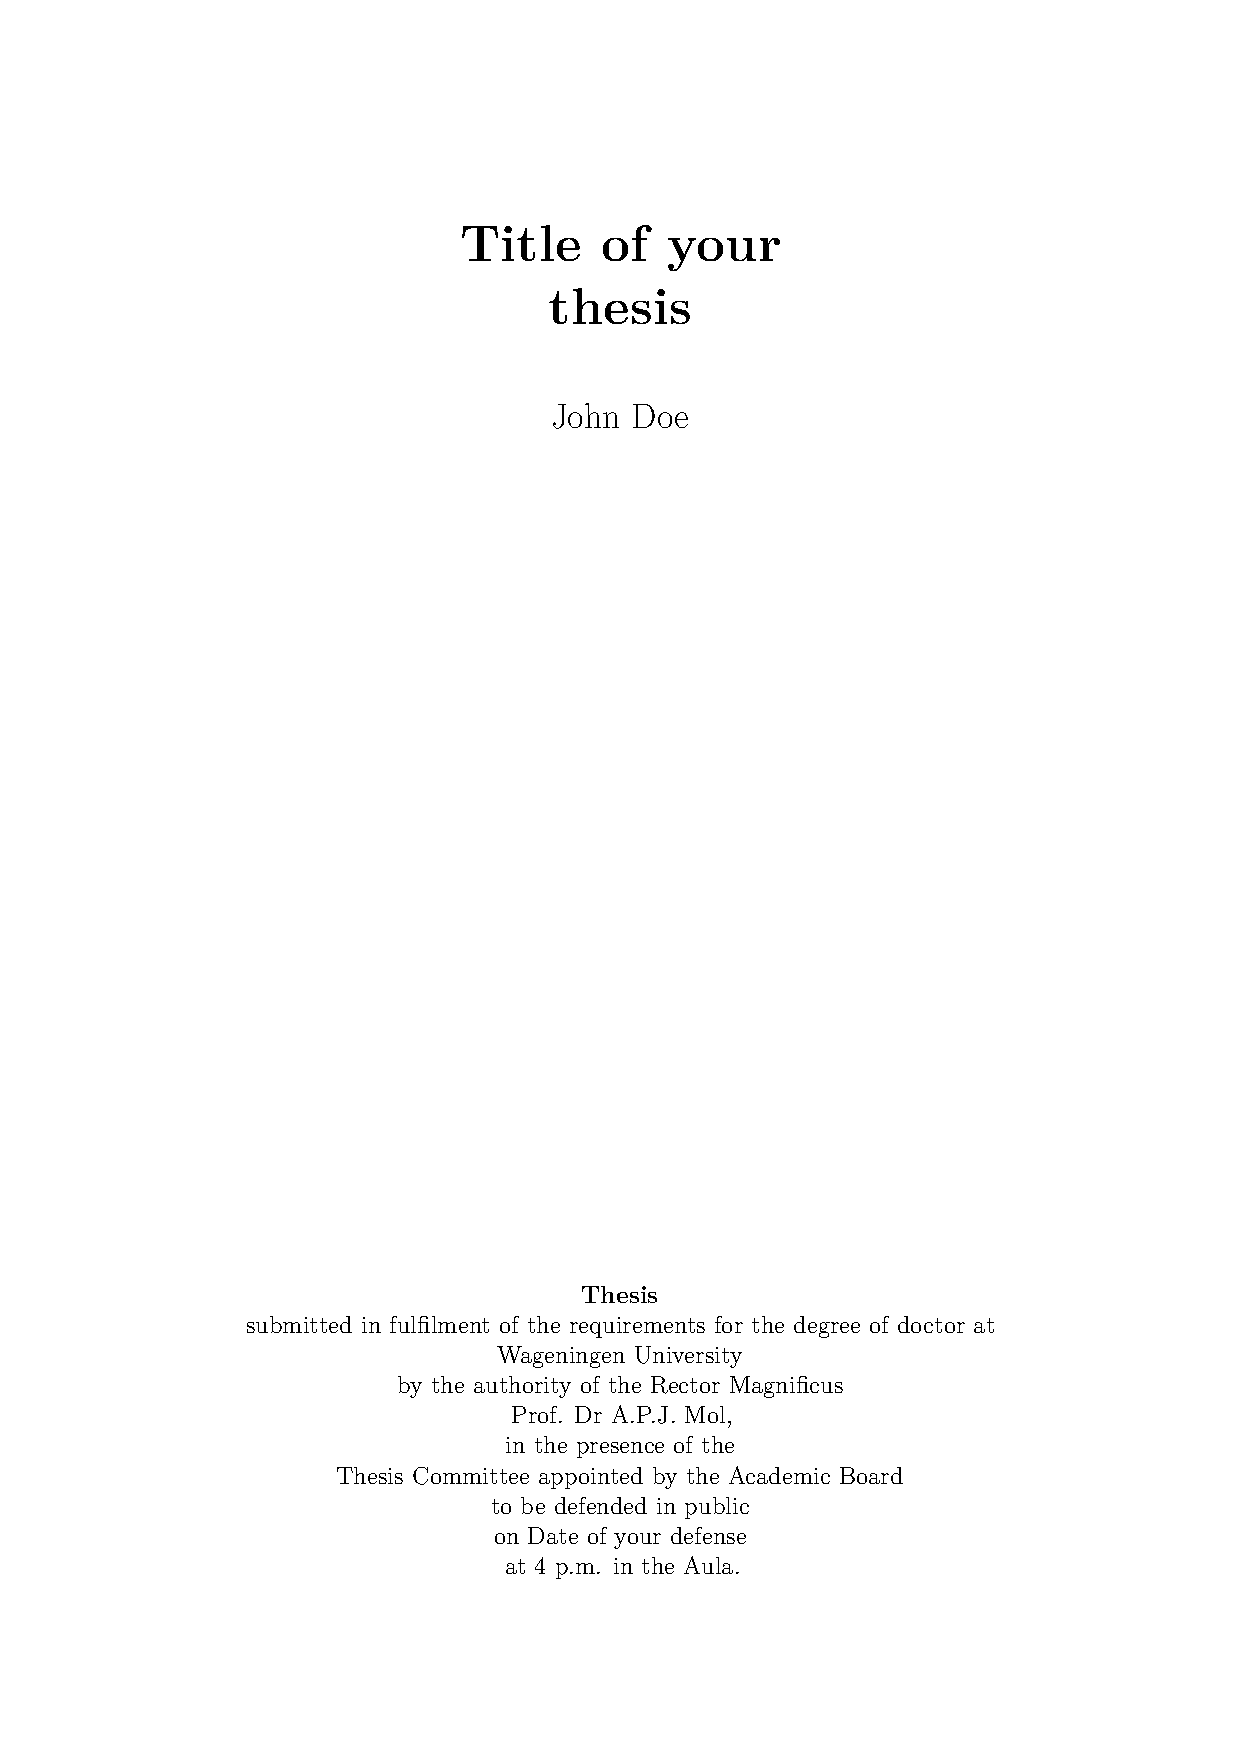
\includegraphics[width=0.32\linewidth]{figures/sample-content/alt_frontmatter_example/split/_000003.pdf}} \fbox{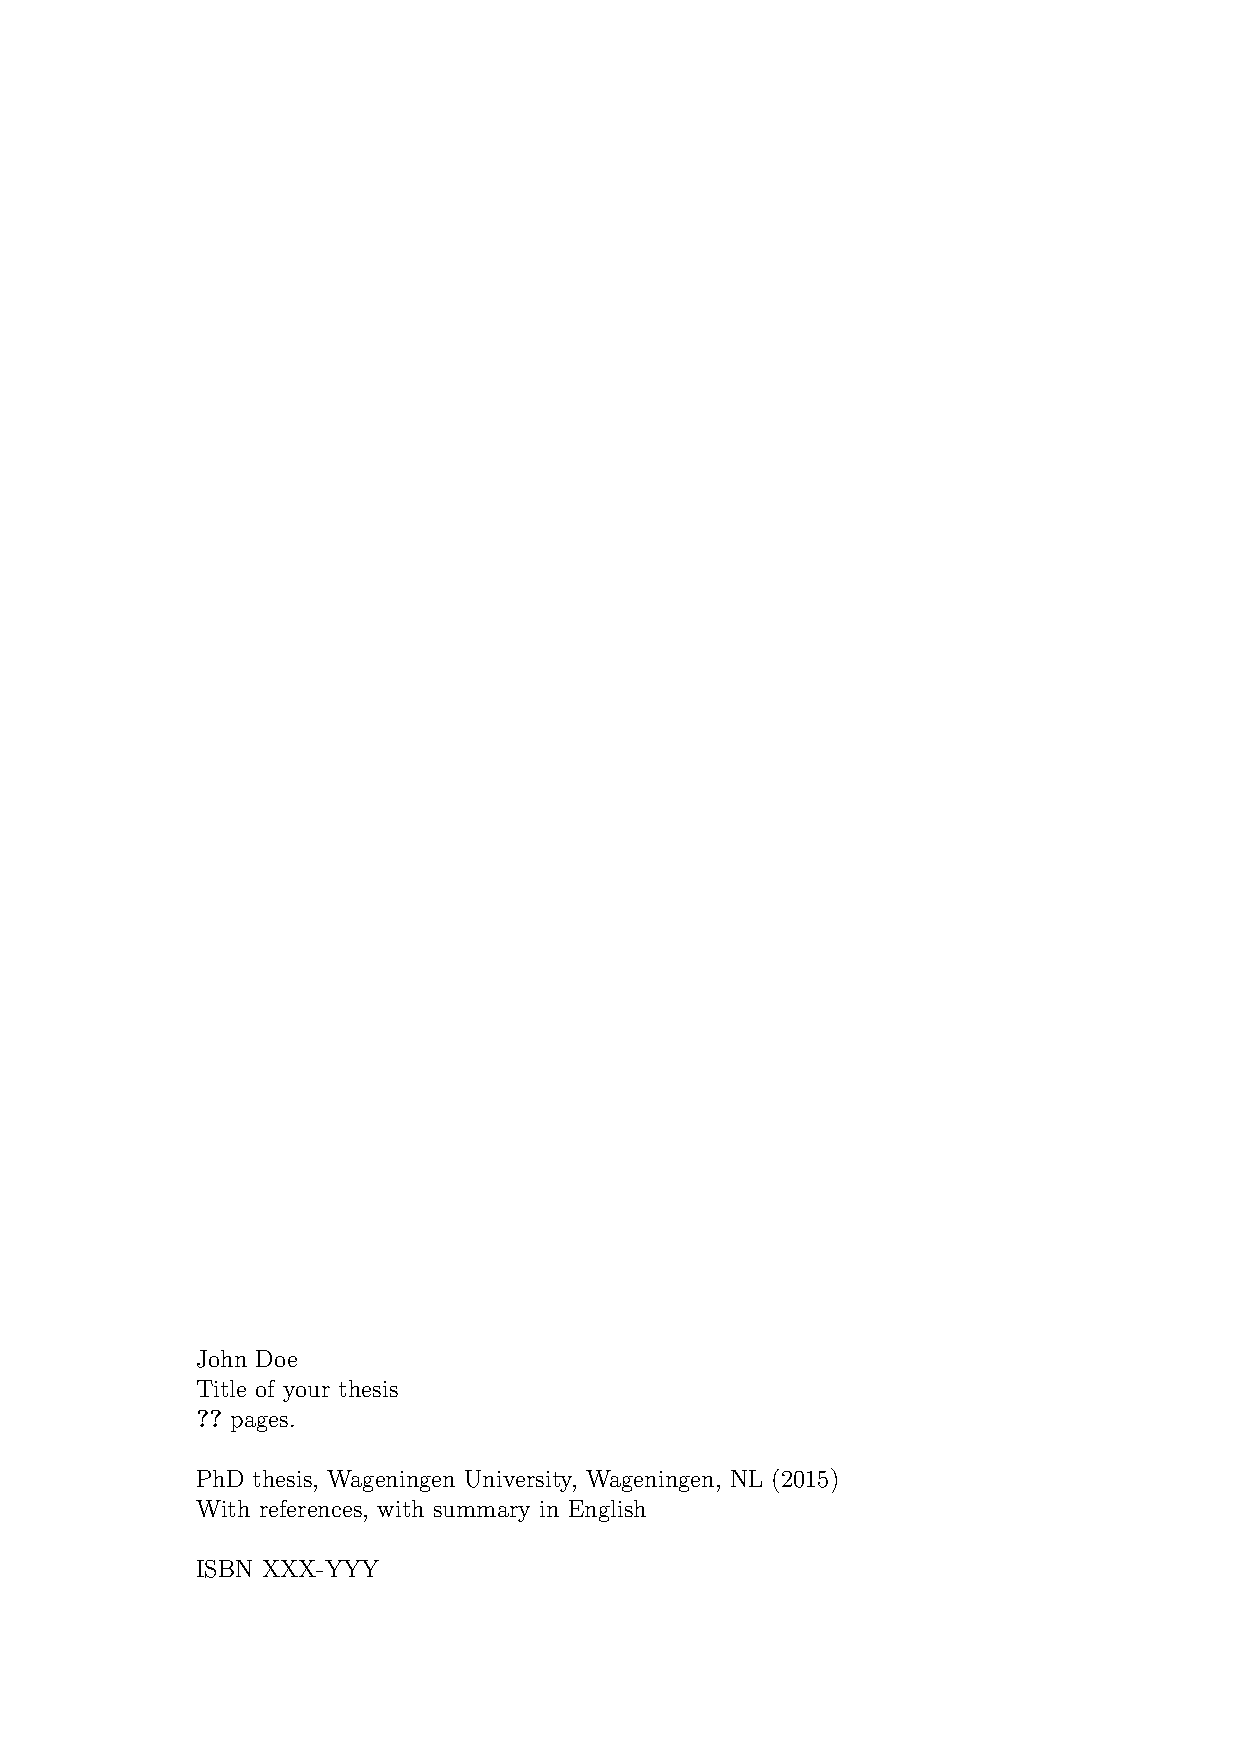
\includegraphics[width=0.32\linewidth]{figures/sample-content/alt_frontmatter_example/split/_000004.pdf}} \fbox{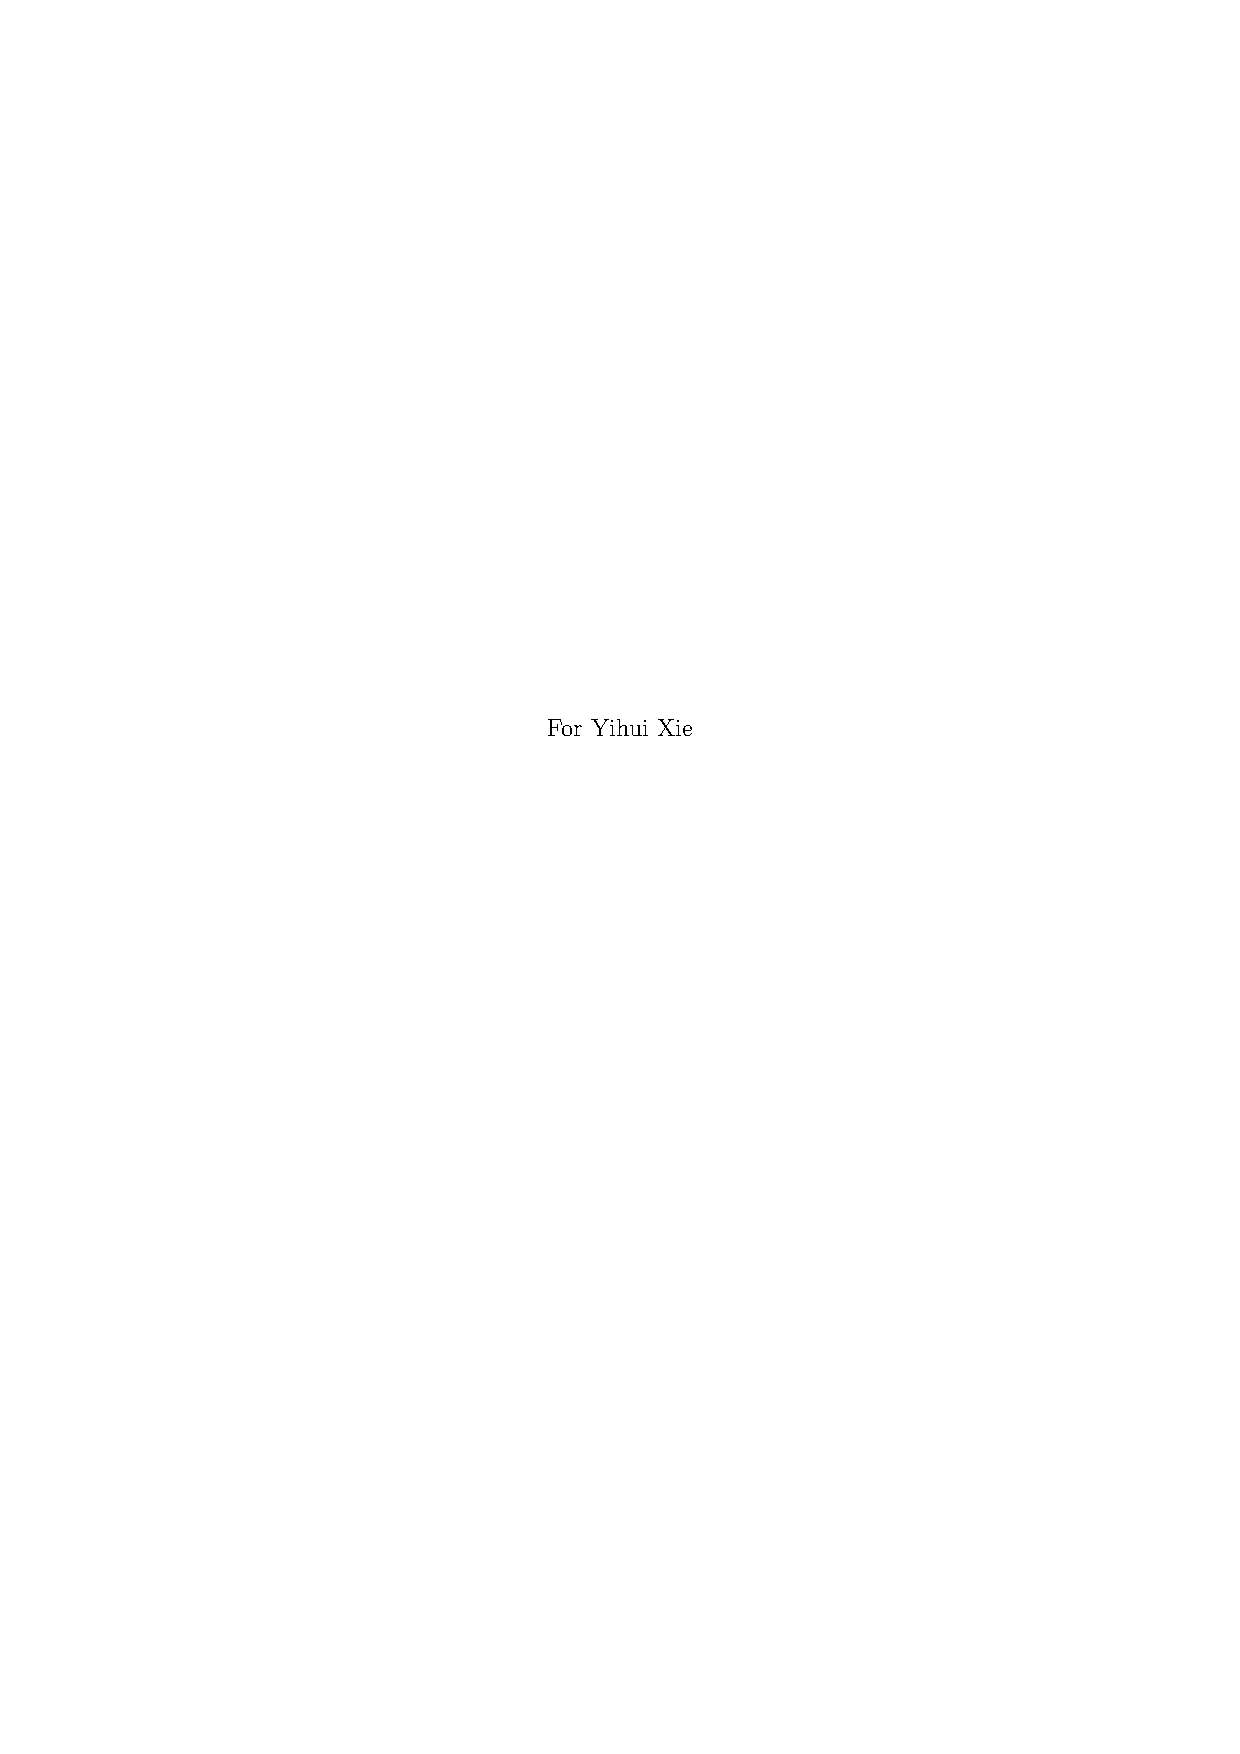
\includegraphics[width=0.32\linewidth]{figures/sample-content/alt_frontmatter_example/split/_000005.pdf}} \fbox{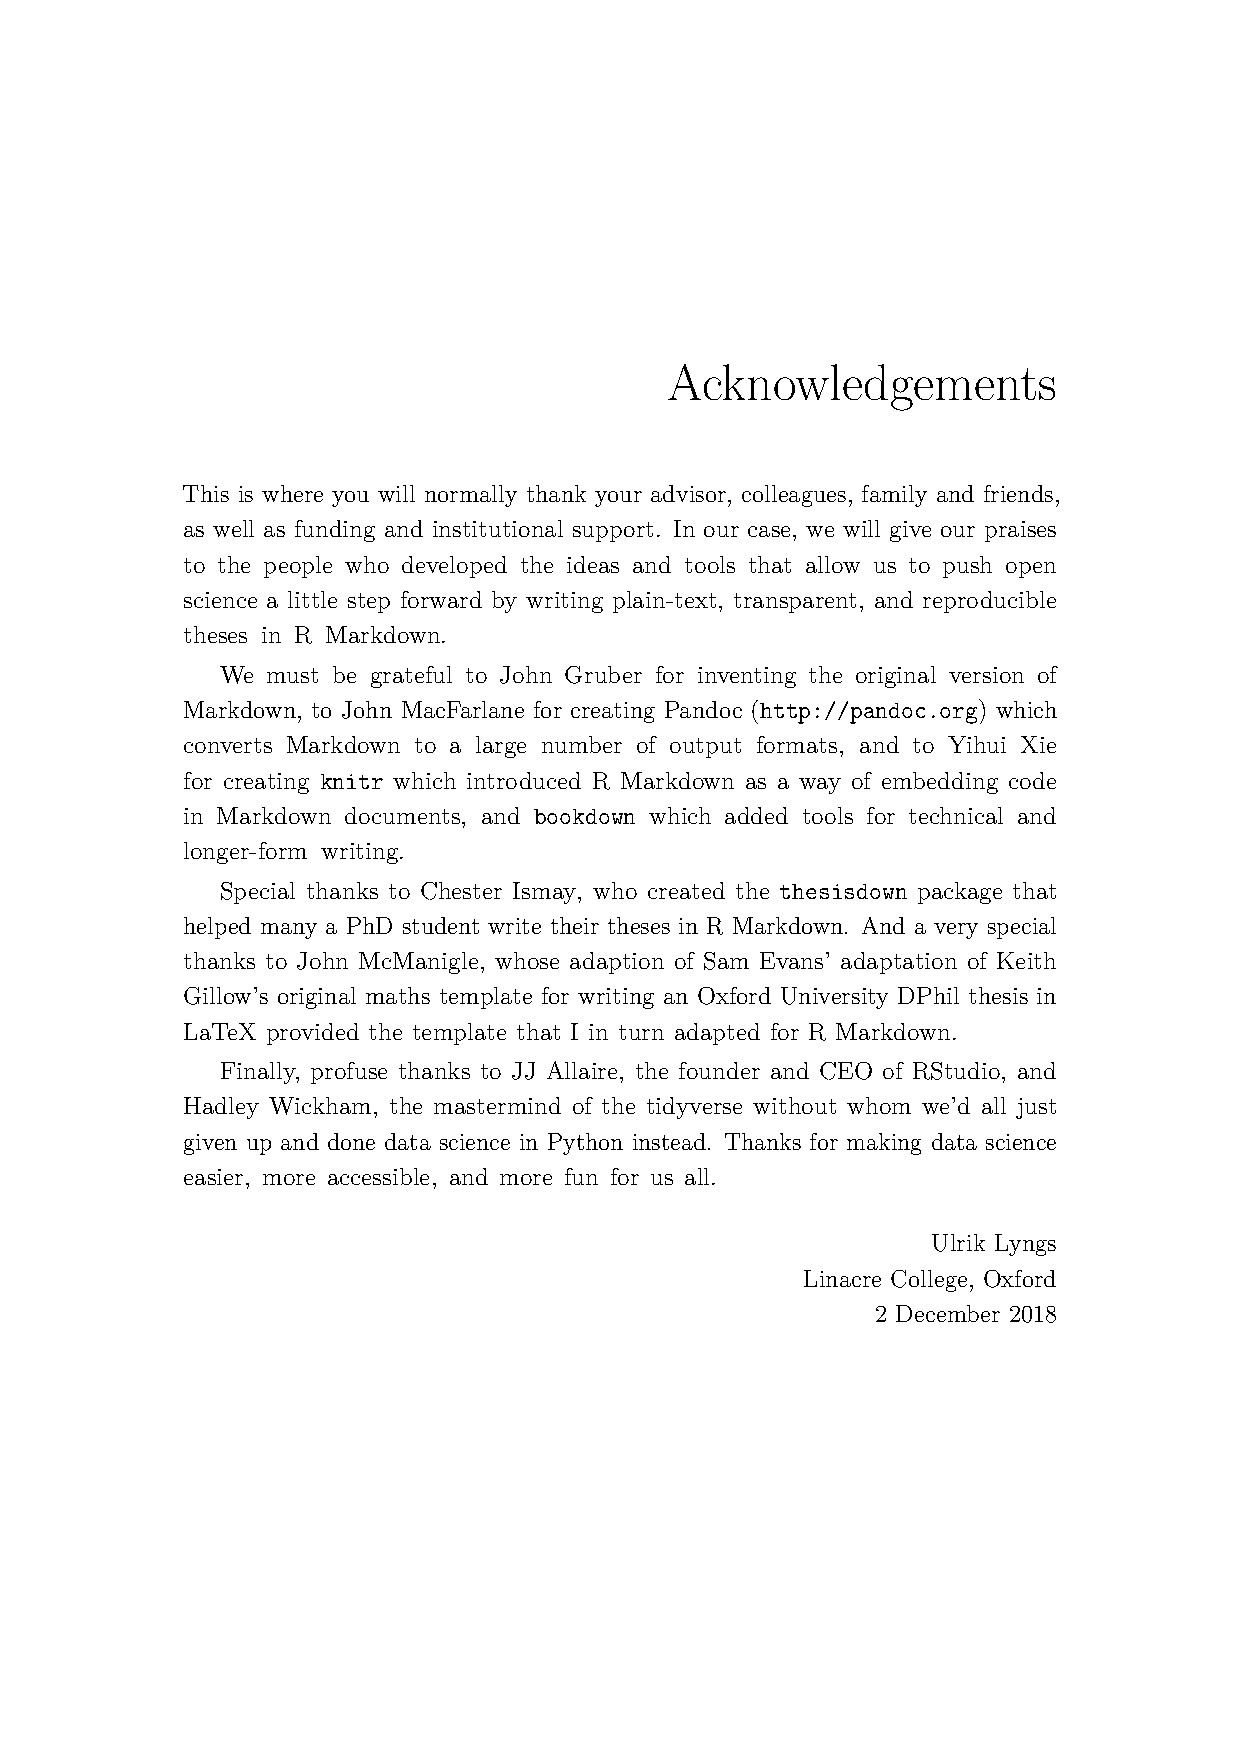
\includegraphics[width=0.32\linewidth]{figures/sample-content/alt_frontmatter_example/split/_000006.pdf}}

\hypertarget{troubleshooting}{%
\chapter{Troubleshooting}\label{troubleshooting}}

This chapter describes common errors you may run into, and how to fix them.

\hypertarget{error-failed-to-build-the-bibliography-via-biber}{%
\section{Error: Failed to build the bibliography via biber}\label{error-failed-to-build-the-bibliography-via-biber}}

This can happen if you've had a failed build, perhaps in relation to RStudio shutting down abruptly.

Try doing this:

\begin{enumerate}
\def\labelenumi{\arabic{enumi}.}
\tightlist
\item
  type \texttt{make\ clean-knits} in the terminal tab (or run \texttt{file.remove(list.files(pattern\ =\ "*.(log\textbar{}mtc\textbar{}maf\textbar{}aux\textbar{}bbl\textbar{}blg\textbar{}xml)"))} in the R console) to clean up files generated by LaTeX during a build
\item
  restart your computer
\end{enumerate}

If this does not solve the problem, try using the \href{https://www.overleaf.com/learn/latex/Bibliography_management_with_natbib}{natbib} LaTeX package instead of \href{https://www.overleaf.com/learn/latex/Articles/Getting_started_with_BibLaTeX}{biblatex} for handling references.
To do this, go to \textbf{index.Rmd} and

\begin{enumerate}
\def\labelenumi{\arabic{enumi}.}
\tightlist
\item
  set \texttt{use-biblatex:\ false} and \texttt{use-natbib:\ true}
\item
  set \texttt{citation\_package:\ natbib} under
\end{enumerate}

\begin{Shaded}
\begin{Highlighting}[]
\FunctionTok{output}\KeywordTok{:}
\AttributeTok{  bookdown:}\FunctionTok{:pdf\_book}\KeywordTok{:}
\AttributeTok{    }\FunctionTok{citation\_package}\KeywordTok{:}\AttributeTok{ natbib}
\end{Highlighting}
\end{Shaded}

\hypertarget{unidade-7}{%
\chapter{Unidade 7}\label{unidade-7}}

\hypertarget{unidade-8}{%
\chapter{Unidade 8}\label{unidade-8}}

\hypertarget{unidade-9}{%
\chapter{Unidade 9}\label{unidade-9}}

\hypertarget{unidade-10}{%
\chapter{Unidade 10}\label{unidade-10}}

\startappendices

\hypertarget{the-first-appendix}{%
\chapter{The First Appendix}\label{the-first-appendix}}

This first appendix includes an R chunk that was hidden in the document (using \texttt{echo\ =\ FALSE}) to help with readibility:

\textbf{In 02-rmd-basics-code.Rmd}

\textbf{And here's another one from the same chapter, i.e.~Chapter \ref{code}:}

\hypertarget{the-second-appendix-for-fun}{%
\chapter{The Second Appendix, for Fun}\label{the-second-appendix-for-fun}}


%%%%% REFERENCES
\setlength{\baselineskip}{0pt} % JEM: Single-space References

{\renewcommand*\MakeUppercase[1]{#1}%
\printbibliography[heading=bibintoc,title={\bibtitle}]}


\end{document}
